% !TeX root=../main.tex
\chapter{مروری بر مطالعات انجام شده}
%\thispagestyle{empty} 
\section{مقدمه}
در مقاله\cite{Nakamoto2009}، در کنار معرفی بیت‌کوین، روشی به نام درستی سنجی پرداخت ساده‌شده (SPV) معرفی شده است. در این روش، امکانی به شبکه بیت‌کوین اضافه گشت که دسته‌ای از کاربران، بدون نیاز به راه‌اندازی یک گره کامل، بتوانند با اثبات مرکلی که از یک گره کامل دریافت می‌کنند، تایید کنند که یک تراکنش درون زنجیره بلوکی بیت‌کوین ثبت گردیده‌ است یا خیر. به این کاربران، کاربر سبک و به گره آن‌ها در شبکه بیت‌کوین، گره سبک گفته می‌شود. گره‌های سبک یا به عبارت دیگر گره‌هایی که در وضعیت تایید ساده‌شده پرداخت‌ها عمل می‌کنند، نیازی به ذخیره تمام زنجیره بلوکی وجود ندارد. این گره‌ها تنها سرایند زنجیره بلوکی را از شبکه دریافت و ذخیره می‌کنند.  هرچند که در این روش کاربران سبک نیاز به بارگیری تمام زنجیره بلوکی بیت‌ کوین را ندارند و تنها لازم است که سرایند بلوک‌ها را ذخیره کنند،‌ اما عملکرد صحیح آن‌ها در گرو ارتباط آن‌ها با یک گره کامل درست کار است. اگرچه گره‌های سبک می‌توانند تایید کنند که سرایند بلوک‌هایی که دریافت کرده‌اند اثبات کار صحیحی دارند یا خیر اما بدون داشتن تمام زنجیره بلوکی نمی‌توانند مطمئن شوند که تمام تراکنش‌های موجود در بلوک‌ها کاملا درست هستند.

آسیب‌پذیری دیگری که گره‌های سبک را تهدید می‌کند، عدم حفظ حریم خصوصی آن‌ها در مقابل گره‌های کاملی است که از آن‌ها درخواست اطلاعات می‌نمایند. یکی از اصلی‌ترین اطلاعاتی که گره‌های سبک از گره‌های کامل درخواست می‌کنند تراکنش‌های مربوط به آدرس(های) گره سبک است. کاربر سبک علاوه بر تراکنش مورد نظر، چکیده بلوکی که تراکنش در آن قرار دارد و همچنین اثبات مرکل وجود آن تراکنش در آن بلوک را دریافت می‌کند. در صورتی که گره سبک به صورت فاش اطلاعات آدرس خود را در اختیار گره کامل قرار دهد، گره کامل خواهد توانست اولا، ارتباط آدرس‌های بیت‌کوین گره سبک با آدرس آی‌پی وی را کشف نماید و در نهایت بفهمد که دارنده این آدرس در کدام موقعیت جغرافیایی قرار دارد (اگر کاربر سبک از شبکه‌های حافظ گم‌نامی استفاده نماید این امکان برای گره کامل وجود نخواهد داشت). ثانیا، این امکان به گره کامل داده می‌شود که بتواند از این طریق ارتباط بین آدرس‌های یک شخص را در شبکه بیت‌کوین ساده‌تر کشف کند. کشف آن که کدام آدرس‌های بیت‌کوین مربوط به یک کاربر به خصوص است، می‌تواند به کشف الگوی رفتاری آن کاربر و در نتیجه کشف نسبی هویت آن منجر شود \cite{Ron2013}. از این رو فاش شدن هر دوی این اطلاعات حریم خصوصی کاربر سبک را نقض خواهد کرد.

به این ترتیب،‌ گره سبک به خاطر اعتماد به یک یا چند گره کامل و نقض حریم خصوصیش از امنیت کمتری نسبت به گره‌های کامل برخوردار است \cite{Sompolinsky2016}. از این رو تاکید می‌شود کاربرانی که مقدار زیادی بیت‌کوین را نگهداری یا مبادله می‌کنند، یا کاربرانی که می‌خواهند گم‌نامی آن‌ها حفظ شود از گره‌ کامل استفاده کنند. با این حال لازم است که تلاش شود امنیت، به ویژه گم‌نامی، کاربران سبک تا حد امکان تامین گردد. چرا که فاش شدن اطلاعات بخشی از اعضای شبکه می‌تواند منجر به فاش شدن اطلاعات دیگر بخش‌های شبکه گردد.

برای حل مشکل فاش شدن آدرس مربوط به گره سبک نزد گره کامل متخاصم، در پروتکل فعلی بیت‌کوین از فیلتر بلوم استفاده می‌شود \cite{Hearn2013}. در مقاله \cite{Gervais2014} توضیح داده ‌شد که استفاده از فیلتر بلوم از امنیت کافی برخوردار نیست. در این فصل پایان‌نامه به معرفی فیلتر بلوم، نحوه استفاده آن در شبکه همتا‌به‌همتای بیت‌کوین و ضعف‌های آن به عنوان ابزاری جهت حفظ حریم خصوصی کاربران خواهیم پرداخت.

\section{تعاریف، اصول و مبانی نظری}



فیلتر بلوم هم اکنون در کیف پول‌هایی نظیر بیت‌کوین‌جِی\RTLfootnote{\lr{Bitcoinj}} \cite{bitcoinj} استفاده می‌شود. در این بخش به معرفی این فیلتر و همچنین نحوه به کارگیری آن در شبکه همتا-به‌همتای بیت‌کوین و آسیب‌پذیری‌های آن پرداخته شده است.

\subsection{بیت‌کوین}

رمزارز بیت‌کوین برای محقق ساختن اهدافی چون تبادل و نگه‌داری دارایی بیت‌کوین بدون نیاز به یک طرف سوم مورد اعتماد از یک الگورتیم اجماع اثبات کار
(PoW\RTLfootnote{Proof of Work})
استفاده می‌کند\cite{Nakamoto2009}. الگوریتم اجماع اثبات کار بیت‌کوین تضمین می‌کند که بدون احتیاج به  وجود یک طرف قابل اعتماد در شبکه، کسی که توان پردازشی آن کمتر از درصد مشخصی از شبکه باشد نتواند حملهٔ دوبار خرج کردن\RTLfootnote{\lr{Double-Spend Attack}}
را اجرا کند.

\subsubsection{بلوک}
%https://developer.bitcoin.org/reference/block_chain.html#block-headers

\subsubsection{تراکنش‌ها و آدرس‌ها‌}
%https://developer.bitcoin.org/reference/transactions.html
بعضی از دادگان ذخیره‌شده در بیت‌کوین به صورت 
اندین کوچک\RTLfootnote{Little-Endian}
ذخیره شده است. که از آن‌ها می‌توان به چکیده‌ها اشاره نمود. در شکل \ref{fig:endian} مقایسهٔ روش اندین کوچک و روش اندین بزرگ \RTLfootnote{Little-Endian} (روشی که انسان‌ها به صورت طبیعی اعداد را می‌خوانند) را برای دادهٔ \lr{\texttt{0x1A2B3C4D5E6F7080}} انجام داده است.

\begin{figure}[h]
	\centering
	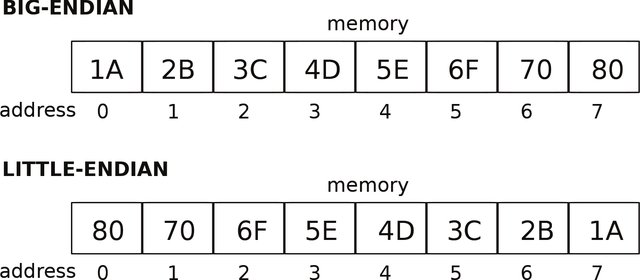
\includegraphics[width=0.7\linewidth]{image/endian}
	\caption{مقایسهٔ اندین کوچک و اندین بزرگ\cite{Grochowski2020}}
	\label{fig:endian}
\end{figure}


\subsubsection{گره‌ها‌}
از روی کتاب Mastering Bitcoin.
تحلیل امنیت‌ هر کدوم از گره‌ها هم ذکر شود.
\paragraph{گره کامل}


\paragraph{گره سبک}

پیاده‌سازی‌های نرم‌افزاری متعددی برای گره سبک یا به عبارت دیگر، کاربر SPV بیت‌کوین وجود دارد. مانند بیت‌کوین‌جی \cite{bitcoinj}، الکترام \RTLfootnote{\lr{Electrum}} 
\cite{Electrum}
و پیکوکوین\RTLfootnote{\lr{PicoCoin}}
\cite{Garzik}. 
اصطلاحا، به نرم‌افزار‌های گره سبک، کیف پول\RTLfootnote{\lr{Wallet}} گفته می‌شود.

بیت‌کوین‌جی یک کتاب‌خانه کاربر سبک (SPV) به زبان جاوا \RTLfootnote{\lr{Java}} است. این کیف پول مستقیما با استفاده از پروتکل‌های ارتباطی استاندارد تعریف شده در شبکهٔ همتا‌به‌همتای بیت‌کوین \cite{P2P_dev,P2P_ref} با گره کامل ارتباط برقرار می‌کند. بیت‌کوین‌جی از اکثر استاندارد‌های بیت‌کوین،‌از جمله فیلتر بلوم \cite{Hearn2013}  پشتیبانی می‌کند. در این پایان‌نامه به صورت کلی منظور از گره سبک یا کاربر \lr{SPV}، بیت‌کوین‌جی است. کاربر سبک بیت‌کوین‌جی به صورت همزمان می‌تواند به چند گره کامل متصل باشد و از طریق آن‌ها اطلاعاتش بروزرسانی گردد.

در پیاده‌سازی الکترام،‌ کاربر سبک مستقیما طبق پروتکل ارتباطی بیت‌کوین با گره کامل مبادلهٔ اطلاعات نمی‌کند. گره کاملی که زنجیره بلوکی بیت‌کوین را ذخیره کرده‌است،‌ لازم است برای ارائه خدمات به کاربران سبکی که از الکترام استفاده می‌کنند،‌ سرور 
الکترام‌ایکس\RTLfootnote{\lr{ElectrumX}}
\cite{ElectrumX}
را در کنار نرم‌افزار گره کامل (هسته‌ٔ بیت‌کون) راه‌اندازی نماید. در این پیاده‌سازی، برخلاف بیت‌کوین‌جی، گره سبک هم‌زمان به چند سرور الکترام‌ایکس متصل نمی‌شود. بلکه به صورت تصادفی یک سرور را انتخاب می‌کند و به آن متصل می‌گردد. کاربر سبک خودش می‌تواند تعیین کند که به چه سروری متصل گردد. از این رو کاربر سبک می‌تواند اطلاعاتش را تنها از گره کاملی که به آن اعتماد دارد به روز رسانی نماید.  همچنین در پروتکل ارتباطی گره سبک الکترام با سرور الکترام‌ایکس از فیلتر بلوم استفاده نمی‌شود. این ویژگی‌ها امنیت این پیاده‌سازی را با ابهام مواجه کرده است \cite{Alison2014}. 

پیکوکوین،‌ یک کتاب‌خانه بیت‌کوین به زبان سی\RTLfootnote{\lr{C}} است. این کتاب‌خانه امکان استفاده به عنوان یک کیف‌پول بیت‌کوین و یک گره کامل را فراهم می‌کند. علاوه بر این، امکان ساخت نرم‌افزارهایی که مرتبط با بیت‌کوین هستند را ممکن می‌کند. این کیف پول از استاندارد ارتباطی بیت‌کوین تبعیت کرده و از فیلتر بلوم استفاده می‌کند، همچنین می‌تواند مستقیما به گره‌های کامل بیت‌کوین، بدون نیاز به راه‌اندازی سروری مجزا در سمت گره کامل، متصل شود.

در این پژوهش هرگاه از گره سبک یا کاربر SPV صحبت می‌شود منظور کیف‌پول بیت‌کوین‌جی \cite{bitcoinj} و هر گاه از گره کامل صحبت می‌شود منظور نرم‌افزار
هستهٔ بیت‌کوین\RTLfootnote{Bitcoin-core} 
\cite{Bitcoincore.org}
است.


\subsubsection{شبکه همتا‌به‌همتای بیت‌کوین}
\label{P2PNetwork}

گره‌های شبکهٔ بیت‌کوین بر اساس یک پروتکل استاندارد با یکدیگر به تبادل پیام می‌پردازند. گره‌های کامل در شبکه بیت‌کوین بعد از آن‌که بلوک‌ها و تراکنش‌های جدید را تصدیق کردند، آن‌ها را به دیگر گره‌ها ارسال می‌کنند. علاوه بر این، گره‌های سبک می‌توانند از پروتکل ارتباطی بیت‌کوین جهت ارتباط با گره‌های کامل استفاده کنند.

تمام  ارتباطات همتا‌به‌همتا در بیت‌کوین در بستر TCP برقرار می‌شوند و تمام پیام‌ها از قالب یکسانی پیروی می‌کنند. رشتهٔ آغازین پیام‌ها و مقدار پیش‌فرض شمارهٔ درگاه با توجه به اینکه پیام در شبکهٔ اصلی، تست یا در حالت تست رگرسیون استفاده می‌شود تفاوت می‌کند. جدول \ref{table:PortandString} این مقادیر را نشان می‌دهد. یک گره می‌تواند از شمارهٔ درگاهی متفاوت در یک شبکه استفاده نماید.



\begin{xltabular}{\textwidth}{|c|c|c|X|}
	\caption{شبکه‌های مختلف بیت‌کوین\label{table:PortandString}}\\
	\hline
	\textbf{شبکه} & \textbf{درگاه پیش‌فرض} & \textbf{رشته‌ٔ آغازین} & \textbf{توضیحات} \\
	\hline \hline 
	اصلی & 8333 & \lr{\texttt{0xf9beb4d9}} & {%
		شبکهٔ اصلی بیت‌کوین.
	}\\
	\lr{Mainnet} & & & {%
		در این شبکه بیت‌کوین دارای ارزش واقعی است.
	} \\
	\hline
	تست & 18333 & \lr{\texttt{0x0b110907}} & {%
		شبکهٔ آزمایشی بیت‌کوین
	}\\
	\lr{Testnet} & & & {%
		برای توسعه دهندگان بهتر و کم هزینه‌ تر است که از شبکهٔ آزمایشی بیت‌کوین استفاده کنند. چرا که بیت‌کوین‌ در آن دارای ارزش واقعی نیست.
	} \\
	\hline
	تست رگرسیون & 18444 & \lr{\texttt{0xfabfb5da}} & {%
		حالت تست رگرسیون
	}\\
	\lr{Regtest} & & & {%
		گاهی در توسعه یک کاربرد نیازی نیست که با گره‌های تصادفی در ارتباط باشیم یا بلوک‌های تصادفی تولید شده را بررسی کنیم. در این شرایط از حالت تست رگرسیون بیت‌کوین استفاده می‌کنیم. در این حالت می‌توان محیط را کنترل کرد و تعیین کرد که چه زمانی یک بلوک جدید ساخته شود.
	} \\
	\hline
	
	
\end{xltabular}


علاوه بر این تمام پیام‌های شبکه‌ٔ همتا‌به‌همتای بیت‌کوین شامل سرایندی یکسان هستند که قالب این سرایند مطابق جدول \ref{table:p2pheader} است.

\begin{xltabular}{\textwidth}{|c|X|}
	\caption{قالب سرایند تمام‌ پیام‌ها در شبکهٔ همتا‌به‌همتای بیت‌کوین \label{table:p2pheader}}\\ \hline
	\textbf{نام} & {\textbf{توضیحات} } \\
	\hline \hline
	\lr{start string}&{%
		بایت‌هایی که در جدول \ref{table:PortandString} توضیح داده شد که نشان دهندهٔ شبکه‌ای است که این پیام در آن تولید شده است.
	}\\
	\hline
	
	\lr{command name} & {%
		رشته‌ای در استاندارد 
		اَسکی\RTLfootnote{ASCII}
		است که مشخص می‌کند چه نوع پیامی در 
		پایه‌بار\RTLfootnote{Payload}
		قرار گرفته است. اندازهٔ این قسمت ۱۲ کاراکتر است و بایت‌های بعد از نام پیام برابر صفر (\texttt{0x00}) خواهند بود. به عنوان مثال برای پیام \texttt{Version} خواهیم داشت:
		\lr{\texttt{version\textbackslash0\textbackslash0\textbackslash0\textbackslash0\textbackslash0}}.
	}\\
	\hline
	
	\lr{payload size} & {%
		اندازه بایت‌های پیام داخل پایه‌بار را مشخص می‌کند. حداکثر تعداد بایت‌ مجاز در پایه‌بار ۳۲ مگابایت‌ (\lr{‍‍``MAX\_SIZE''}) است. پیام‌های بزرگ‌تر از این مقدار دورانداخته می‌شوند. پیام‌هایی مانند \texttt{VerAck}   بدون پایه‌بار هستند.
	}\\
	\hline
	
	\lr{checksum} & {%
		چهار بایت اول حاصل 
		\lr{SHA256(SHA256(payload))}
		است. اگر پایه‌بار خالی باشد، مانند پیام‌های \texttt{VerAck} و \texttt{GetAddr}، مقدار این بخش برابر 
		\lr{\texttt{0x5df6e0e2}}
		بوده که معادل 
		\lr{SHA256(SHA256(
			\rl{رشتهٔ خالی}
			))}
		است.
	}\\
	\hline
	
\end{xltabular}  

\paragraph{یافتن همتا}

اولین گامی که هر گره در شبکهٔ همتا‌به‌همتای بیت‌کوین انجام می‌دهد، یافتن گره‌های (همتا‌های) دیگر و اتصال به آن‌ها است. از آن‌جایی که یک گره در زمان راه اندازی، آدرس آی‌پی گره‌های کامل فعال را ندارد، از یک یا چند سرور 
\RTLfootnote{\lr{Domain Name System}}\lr{DNS} 
که آدرس‌ آن‌ها در کد بیت‌کوین‌جی از پیش قرارگرفته است پرسمان انجام می‌دهد. پاسخ دریافت شده شامل آدرس یک یا چند گره کامل است که ارتباطات ورودی را قبول می‌کنند. علاوه بر این تعدادی آدرس گره کامل در کدهای بیت‌کوین‌جی قرار دارد که در زمانی که یک ورژن مشخص منتشر می‌شده فعال بوده‌اند. 
\paragraph{اتصال به همتا}
بعد از آن‌که کاربر جدید آدرس آی‌پی یک یا چند گره کامل را بدست آورد، برای آن گره‌(ها) پیام \texttt{version} را ارسال می‌کند. این پیام برای ایجاد ارتباط ارسال می‌شود و شامل اطلاعاتی از گره ارسال کننده است. این اطلاعات در جدول \ref{table:VersionMessage} توضیح داده شده است. گره دریافت کننده نیز یک پیام \texttt{version} را که شامل اطلاعات خودش است، ارسال می‌کند. هر دو گره به محض دریافت پیام \texttt{version} پیام \texttt{verack} را برای گره مقابل ارسال می‌نماید. پیام \texttt{verack} بدون
پایه‌بار\RTLfootnote{Payload}
است و به گره دریافت کننده اطلاع می‌دهد که آماده دریافت پیام‌‌های بعدی است.


\begin{xltabular}{\textwidth}{|c|X|}
	\caption{
		قسمت‌های پیام \texttt{version} در شبکه همتا‌به‌همتای بیت‌کوین
		\label{table:VersionMessage}}\\
	\hline
	\textbf{نام} & {\centering
		\textbf{توضیحات}		
	} \\
	\hline
	\hline
	\lr{version} & {
		بالاترین نسخهٔ پروتکلی که توسط گره ارسال کننده شناخته می‌شود.	در زمان نگارش این پایان‌نامه، بالاترین نسخه پروتکل بیت‌کوین 70015 است که در سال ۲۰۱۷ منتشر شده است.
	} \\
	\hline
	\lr{services} & {
		خدماتی که گره ارسال‌کننده پشتیبانی می‌کند را مشخص می‌کند. برای گره‌های سبکی مثل بیت‌کوین‌جی، مقدار آن برابر \texttt{0x00} است.
	} \\
	\hline
	\lr{timestamp} & {
		ساعت یونیکس\RTLfootnote{\lr{Unix time}} با توجه به ساعت گره ارسال کننده در زمان ارسال پیام.
	} \\
	\hline
	\lr{addr\_recv services} & {
		سرویس‌هایی که از دید گره ارسال‌کننده، توسط گره گیرنده پشتیبانی می‌شود. فرمت نمایش آن مانند قسمت services است. اگر گره ارسال‌کننده، بیت‌کوین‌جی باشد، همیشه به صورت پیش‌فرض مقدار این قسمت را برابر \texttt{0x00} قرار می‌دهد.
	} \\
	\hline
	\lr{addr\_recv port} & {
		شماره پورت گره گیرنده از دید گره ارسال‌کننده.
	}\\
	\hline
	\lr{addr\_trans services} & {
		خدماتی که گره ارسال‌کننده پشتیبانی می‌کند را مشخص می‌کند. یکسان با قسمت services باید باشد.
	}\\
	
	\hline
	\lr{addr\_trans IP address} & {
		آدرس آی‌پی گره ارسال کننده.
	}\\
	
	\hline
	\lr{addr\_trans port} & {
		شماره پورت گره ارسال کننده.
	}\\
	
	\hline
	\lr{nonce} & {
		تک‌شمار، یک عدد تصادفی است که اگر یک گره،‌ یک پیام با تک‌شماری مشابه با تک‌شمار ارسالی دریافت کرد، ارتباط را قطع نماید. (قسمت تک‌شمار در نسخهٔ \lr{$0.1.6$} بیت‌کوین اضافه شده و هدفش آن است که گره متوجه شود که به خودش متصل نشده است)
		\RTLfootnote{  \lr{\url{https://github.com/bitcoin/bitcoin/commit/cc0b4c3b62367a2aebe5fc1f4d0ed4b97e9c2ac9}}}.
	}\\
	\hline
	\lr{user\_agent bytes} & {
		تعداد بایت‌هایی که قسمت \lr{user\_agent} (قسمت بعدی) استفاده کرده است.
	}\\
	
	\hline
	\lr{user\_agent} & {
		نوع برنامه کاربر را معین می‌کند. مثلا:
	}\\
	
	&  {%
		۱. بیت‌کوین‌جی: 
		\lr{/bitcoinj:1.0/MultiBit:1.0(Windows)/}} \\
	&  {%
		۲. هستهٔ بیت‌کوین (گره کامل): 
		\lr{/Satoshi:0.20.0/(70015)/}} \\
	
	\hline
	\lr{start\_height} & {
		ارتفاع بهترین زنجیره‌ بلوکی گره ارسال کننده در این قسمت قرار گرفته می‌شود. در صورتی که کاربر SPV باشد، ارتفاع بهترین زنجیره سرایند بلوک‌‌ها قرار داده می‌شود.
	}\\
	
	\hline
	\lr{relay} & {
		قرار دادن این بخش در پیام اختیاری است. این بخش در \cite{Hearn2013} به همراه پیشنهاد استفاده از فیلتر بلوم در بیت‌کوین معرفی شده است. مقدار آن صحیح (\texttt{0x01}) یا غلط (\texttt{0x00}) است. در صورتی که صحیح باشد، یا از آن استفاده نشود، تغییری در پروتکل ایجاد نمی‌شود. ولی در صورتی که غلط باشد، قبل از آن‌که کاربر ارسال کننده، پیام‌های \texttt{filterload} و \texttt{filterclear} را ارسال کرده باشد، هیچ پیام \texttt{inv} یا \texttt{tx} به آن ارسال نمی‌شود. این کار باعث می‌شود که در فاصلهٔ زمانی انجام 
		دستداد \RTLfootnote{Handshake}
		(ارسال پیام \texttt{version}) و فرستادن فیلتر بلوم، کاربر سبک تحت سیل پیام‌های گره‌کامل اشباع نشود. 
	}\\
	
	
	\hline
\end{xltabular}

زمانی که اتصال با یک گره کامل برقرار شد، پیام \texttt{getaddr} برای گره کامل فرستاده می‌شود تا آدرس آی‌پی گره‌های کامل فعالی که گره دریافت‌کننده به آن‌ها متصل است در قالب پیام \texttt{addr} برای گره فرستنده ارسال شود. گره فرستنده همتا‌های فعال خودش را نیز در قالب پیام \texttt{addr} برای گره کامل گیرنده ارسال می‌کند.

\paragraph{هم‌گام سازی}
کاربر سبک بعد از اتصال اولیه به یک گره کامل، نیاز دارد که سرایند بلوک‌های زنجیرهٔ بلوکی را دریافت نماید به این کار 
هم‌گام‌سازی \RTLfootnote{Synchronization}
 گفته می‌شود. همان‌طور که گفته شد کاربر سبک به جای ذخیره‌سازی و تصدیق تمام زنجیرهٔ بلوکی،‌ تنها سرایند آن را ذخیره می‌کند. حجم سرایند یک بلوک $80$ بایت است. در گره‌های کامل، که می‌خواهند تمام زنجیره بلوکی را دریافت نمایند، این فرایند به دو صورت
«ابتدا-بلوک\RTLfootnote{Blocks-First}»
یا
«ابتدا-سرایند\RTLfootnote{Headers-First}»
قابل انجام است که در این‌جا به توضیح آن‌ها پرداخته نمی‌شود. گره سبک در گام اول هم‌گام‌سازی لازم است که بهترین سراید زنجیرهٔ بلوکی \RTLfootnote{\lr{Best header chain}} را دانلود کند. سرایند زنجیرهٔ بلوکی، زنجیره‌ای از سرایند بلوک‌ها است که هر کدام از سرایند‌ها به سرایند بلوک قبل خود اشاره می‌کند. بهترین سرایند زنجیرهٔ بلوکی، زنجیره‌ای است که دشوارترین بازآفرینی را داشته باشد. 

گره سبک برای دریافت سرایند زنجیرهٔ بلوکی، پیام \texttt{getheaders} را برای گره کاملی (گره هم‌گام‌ساز) که می‌خواهد با آن همگام شود ارسال می‌کند. جدول \ref{table:GetHeadersMessage} بخش‌های مختلف این پیام را توضیح می‌دهد و شکل \ref{fig:getheaders} مثالی از یک پیام \texttt{getheaders} است که گره سبک برای اولین‌بار برای گره هم‌گام‌ساز ارسال می‌کند.



\begin{xltabular}{\textwidth}{|c|X|}
	\caption{
		قسمت‌های پیام \texttt{getheaders} در شبکه همتا‌به‌همتای بیت‌کوین
		\label{table:GetHeadersMessage}}\\
	\hline
	\textbf{نام} & {\textbf{توضیحات}} \\
	\hline \hline
	\lr{version} & {%
		شماره‌ٔ نسخه‌ٔ پروتکل. شبیه آنچه در پیام \texttt{version} ارسال شد.
	} \\
	
	\hline
	
	\lr{hash count} & {%
		تعداد چکیده‌هایی که در بخش بعدی پیام قرار می‌گیرند، در این قسمت تعیین می‌شوند. محدودیتی در تعداد چکیده‌های ارسالی نیست. اما اندازه کل پیام باید کمتر از \lr{‍‍``MAX\_SIZE''} (۳۲ مگابایت) باشد.
	} \\
	\hline
	
	
	\lr{block header hashes} & {%
		چکیدهٔ یک یا چند سرایند بلوکی که گره ارسال کننده آن‌ها را در حافظهٔ خود دارد. ترتیب چکیده‌ها از بالاترین ارتفاع بلوک (جدید‌ترین) به پایین‌ترین ارتفاع است. به این ترتیب به گره دریافت‌کننده‌ٔ پیام این امکان داده می‌شود که جدیدترین چکیدهٔ سرایندی که با هم مشترک هستند را پیدا کند. اگر گره ارسال‌کننده تازه راه‌اندازی شده‌ باشد در این قسمت، چکیدهٔ بلوک جنسیس (\lr{6fe2…0000}) را که در نرم‌افزارش از ابتدا وجود داشته است، قرار می‌دهد.
	} \\
	\hline
	
	\lr{stop hash} & {%
		این قسمت چکیدهٔ آخرین بلوکی است که گره ارسال‌کننده می‌خواهد دریافت کند. با صفر قراردادن آن، حداکثر پاسخ ممکن از گره دریافت‌کننده تقاضا می‌شود. حداکثر تعداد سرایندی که گره کامل دریافت کننده پاسخ دهد، $2000$ سرایند است. 
	}\\
	\hline
	
\end{xltabular}

\begin{figure}[h]
	\centering
	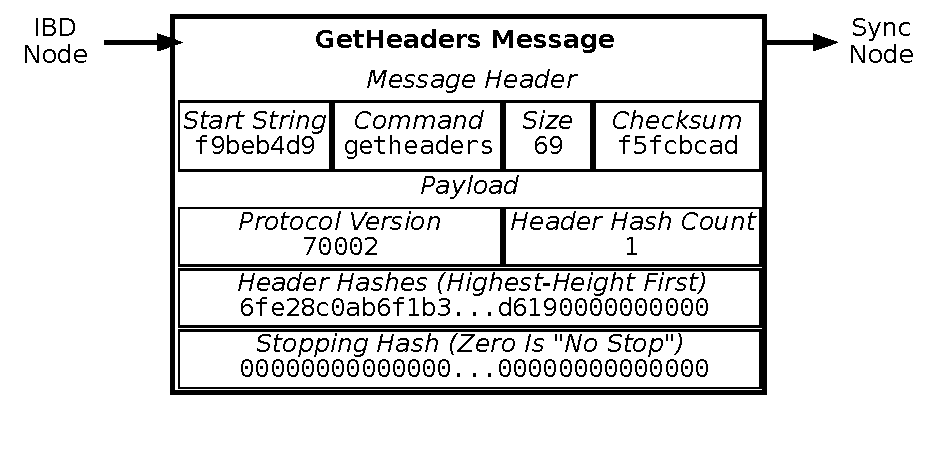
\includegraphics[width=0.7\linewidth]{image/getheaders}
	\caption{مثالی از پیام \texttt{getheaders} در همگام‌سازی اولیهٔ یک گره جدید}
	\label{fig:getheaders}
\end{figure}


گره هم‌گام‌ساز در پاسخ به پیام \texttt{getheaders} در شکل \ref{fig:getheaders} دنبال بلوکی با چکیده مشخص شده می‌گردد و می‌یابد که این بلوک برابر بلوک شمارهٔ صفر (بلوک جنسیس) است. به این ترتیب $۲۰۰۰$ سرایند بلوک را که از بلوک شمارهٔ یک آغاز می‌شوند در قالب پیام \texttt{headers} برای گره درخواست دهنده ارسال می‌کند. قالب این پیام در جدول \ref{table:HeadersMessage} مشخص شده‌ است. شکل \ref{fig:headers} مثالی از پیام بازگردانده شده توسط گره هم‌گام‌ساز است.

\begin{table}[!h]
	\centering
	\caption{
		قسمت‌های پیام \texttt{headers} در شبکه همتا‌به‌همتای بیت‌کوین
		\label{table:HeadersMessage}}
	\begin{tabular}{|c|r|}
		\hline
		\textbf{نام} & {\textbf{توضیحات}} \\
		\hline \hline
		
		\lr{count} & {%
			تعداد سرایند‌های بلوک قرار گرفته در بخش بعدی این پیام. (حداکثر $2000$)
		} \\
		\hline
		
		\lr{headers} & {%
			سرایند‌ بلوک‌ها در این قسمت قرار می‌گیرند.
		} \\
		\hline
	\end{tabular}
\end{table}

\begin{figure}[!h]
	\centering
	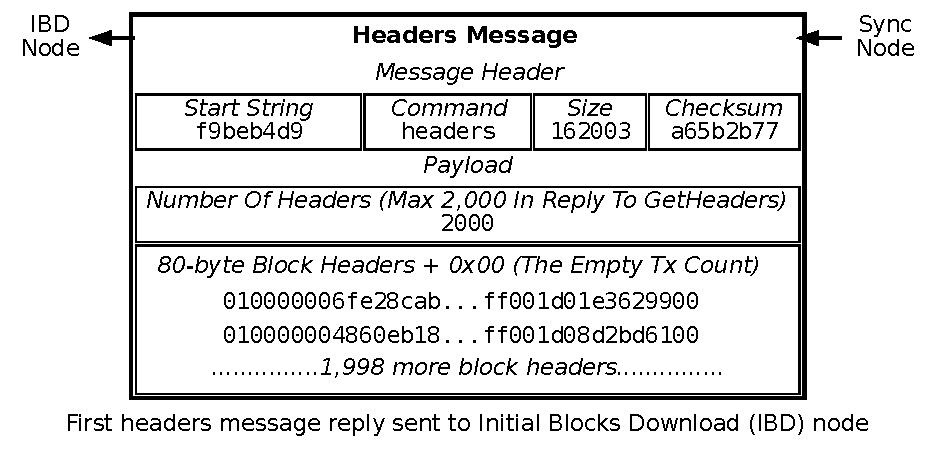
\includegraphics[width=0.7\linewidth]{image/headers}
	\caption{مثالی از پیام \texttt{headers} در همگام‌سازی اولیهٔ یک گره جدید}
	\label{fig:headers}
\end{figure}

وقتی گره سبک پاسخ شکل \ref{fig:headers} را دریافت کرد، فورا صحت آن را بررسی کرده و مجددا پیام  \texttt{getheaders} جدیدی برای گره همگام‌ساز برای گرفته باقیمانده سرایند‌ها ارسال می‌کند. این فرایند تا گرفتن کامل سرایند‌ها ادامه پیدا می‌کند. در زمان نوشتن این پایان‌نامه، حجم تمام سرایند‌های زنجیرهٔ بلوکی ۵۰ مگابایت است. پس از اتمام دانلود سرایند‌های زنجیرهٔ  بلوکی، گره سبک آخرین پیام \texttt{getheaders} را برای چند همتای دیگر ارسال می‌کند و پاسخ آن‌ها را با پاسخ گره هم‌گام‌ساز ابتدایی مقایسه می‌کند. به این ترتیب مطمئن می‌شود که بهترین سرایند زنجیرهٔ بلوکی را دریافت کرده است. 

\paragraph{انتشار}

زمامی که گره کامل یک بلوک جدید را دریافت می‌کند، پیام \texttt{inv} را برای همهٔ همتا‌هایش (چه گره کامل چه گره سبک) ارسال می‌کند. پیام ارسال شده دارای یک 
مدخل فهرست \RTLfootnote{Inventory} 
مربوط به بلوک جدید است. یک مدخل فهرست، شامل یک علامت نوع داده و یک  چکیده داده به عنوان مشخص‌کنندهٔ آن است. داده می‌تواند انواع مختلفی داشته باشد، به عنوان نمونه، علامت تراکنش
\lr{``MSG\_TX''}
و علامت بلوک
\lr{``MSG\_BLOCK''}
است.
 به صورت کلی مدخل فهرست به وجود تراکنش‌ها یا بلوک‌هایی برای دانلود اشاره می‌کند. جدول \ref{table:InvMessage} قسمت‌های مختلف پیام \texttt{inv} را شرح می‌دهد. 

\begin{xltabular}{\textwidth}{|c|X|}
	\caption{
		قسمت‌های پیام \texttt{inv} در شبکه همتا‌به‌همتای بیت‌کوین
		\label{table:InvMessage}}\\
	\hline
	\textbf{نام} & {\textbf{توضیحات}} \\
	\hline \hline
	
	\lr{compactSize uint} & {%
	تعداد مدخل‌های فهرست. 
}\\
\hline

	\lr{inventory} & {%
	یک یا چند مدخل فهرست. حداکثر تعداد آن می‌تواند $50000$ باشد. به عنوان مثال محتوای این قسمت از پیام برای اطلاع‌رسانی بلوک ارتفاع 
	$645747$\RTLfootnote{\url{https://blockchair.com/bitcoin/block/645747}}
	به گره‌های همتا به این صورت است: 
}\\

&{%
علامت نوع داده:
\lr{MSG\_BLOCK}
}\\

&{%
مشخص‌کنندهٔ داده (چکیده):
\lr{\texttt{0x333ab9f10d...0000000000}}
}\\

\hline

\end{xltabular}

گره سبک بعد از دریافت این پیام، یک پیام \texttt{getdata} برای گره کامل می‌فرستد. در این پیام درخواست می‌کند که با توجه به فیلتر بلومی که پیش‌تر در اختیار گره کامل گذاشته بوده، تراکنش‌هایی از بلوک جدید را، که در آن فیلتر صدق می‌کنند برای اون بفرستد. ساختار پیام \texttt{getdata} شبیه \texttt{inv} است. با این تفاوت که علامت نوع داده،‌ اطلاعاتی است که گره ارسال کننده این پیام از گره دریافت‌کننده درخواست می‌کند. 
در این کاربرد، گره سبک علامت \lr{‍‍‍``MSG\_FILTERED\_BLOCK''}  را در کنار چکیده‌ٔ بلوک مورد نظر در پیام قرار می‌دهد و برای گره کامل ارسال می‌کند. به این ترتیب گره کامل تراکنش‌هایی که حداقل یک آدرس آن‌ها در فیلتر بلوم صدق می‌کنند را در کنار اثبات مرکل آن‌ها برای گره سبک ارسال می‌کند.
پاسخ در قالب یک پیام \texttt{merkleblock} که شامل اثبات مرکل وجود تراکنش‌های مرتبط در بلوک است و تعداد صفر یا چند پیام \texttt{tx} را که خود تراکنش‌ها هستند خواهد بود. 

به خاطر ماهیت فیلتر بلوم، پاسخ گره کامل  شامل تراکنش‌هایی می‌شود که مورد توجه گره سبک نیستند. این اتفاق منجر به گمراه شدن گره کامل در شناخت تراکنش‌های مرتبط با گره سبک می‌شود. هدف از این کار حفظ گم‌نامی کاربر سبک و فاش نشدن آدرس وی نزد گره کامل است. در قسمت \ref{BloomFilter} علاوه بر توضیح فیلتر بلوم، نحوه استفاده از آن در شبکهٔ همتابه‌همتا، مثل ارسال آن برای گره کامل  از طریق ارسال پیام \texttt{filterload} و نحوهٔ تولید پیام \texttt{merkleblock}  توسط گره کامل و ساختار آن توضیح داده می‌شود. همچنین، در این قسمت در مورد آسیب‌پذیری‌های فیلتر بلوم و ناتوانی آن در حفظ حریم خصوصی کاربران بحث خواهد شد.


\subsection{فیلتر بلوم}
\label{BloomFilter}
فیلتر بلوم را نخستین بار برتون بلوم در \cite{Bloom1970} معرفی کرد. هدف این فیلتر امتحان سریع وجود یک عضو در یک مجموعه است. فیلتر بلوم کاربرد گسترده‌ای در پایگاه‌های داده، شبکه و حتی موتور‌های جست‌وجو دارد. فیلتر بلوم آرایه‌ای از $n$ بیت $b[i]$ است که $i$ از $0$ تا$n-1$ است. به صورت پیش‌فرض تمام بیت‌ها مقدار صفر دارند. اگر بخواهیم عضو $x$ را (مثلا یک رشته) درون مجموعه آن قرار دهیم، آن عضو را در ورودی $k$ تابع چکیده‌ساز مستقل
$H_1(.), H_2(.), ..., H_k(.)$
قرار می‌دهیم. خروجی هر تابع چکیده ساز یک عدد صحیح بین $0$ تا $n-1$ است. از این رو هر تابع چکیده ساز، یک عنصر ورودی را به یکی از	 $n$ بیت فیلتر بلوم نگاشت می‌کند. برای قرار دادن آن رشته در مجموعه مربوط به فیلتر بلوم، بیت متناظر عدد حاصل را برابر با یک قرار می‌دهیم: 

$\forall j\in \{1..k\}, b[H_j(x)] \leftarrow 1$.

به همین ترتیب اگر بخواهیم بررسی کنیم که یک رشته در مجموعه قرار دارد، چکیده آن رشته را توسط همان $k$ تابع چکیده‌ساز حساب نموده و بررسی می‌کنیم که آیا مقدار ذخیره شده در تمام $k$ جایگاه بدست آمده برابر یک است یا خیر. اگر برابر با یک باشد، آن رشته را عضو احتمالی آن مجموعه در نظر می‌گیریم. به آن عضو احتمالی گفته می‌شود چرا که ممکن است عناصری عضو مجموعه نباشند و به جایگاه‌هایی که مقدار  بیت آن‌ها برابر با یک است نگاشت شوند. به این ترتیب امکان بروز خطای نوع دو وجود دارد. مجموعهٔ تمامی عناصر با $\mathcal{U}$، اعضایی که درون فیلتر بلوم قرار گرفته‌اند با $\mathcal{S}$ و مجموعهٔ عناصری که در نتیجه خطای نوع دو عضو فیلتر بلوم در نظر گرفته می‌شوند با $\mathcal{V}$ نمایش داده می‌شوند. به صورت کلی می‌توان گفت هرگاه لیست یا مجموعه‌ای مورد استفاده قرار گرفت، هزینه فضای ذخیره‌سازی و دسترسی به اعضای مجموعه قابل توجه بود و خطای نوع دو خسارت و هزینه چندانی به سامانه تحمیل نکند، استفاده از فیلتر بلوم مفید خواهد بود. فیلتر بلوم امکان انجام مصالحه بین فضای استفاده شده، زمان پاسخ‌گویی و احتمال خطای قابل قبول را فراهم می‌کند\cite{Bloom1970}. با توجه به ساختار فیلتر بلوم روشن است که امکان بروز خطای نوع یک، یا به عبارت دیگر امکان آنکه عضو مجموعه را غیر عضو تشخیص دهد، وجود ندارد.

\begin{figure}
	\centering
	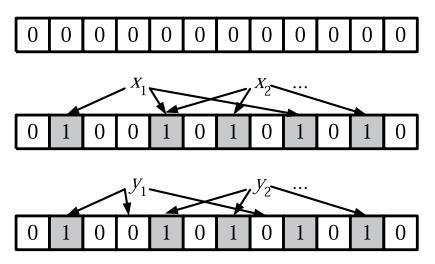
\includegraphics[width=0.55\linewidth]{image/BloomFilter}
	\caption[نمونه‌ای از عمکلرد فیلتر بلوم]{
		فیلتر مجموعه بدون عضو متشکل از یک آرایه‌ از بیت‌ها با مقدار صفر است. k دفعه چکیده هر عضو مجموعه $x_i$ محاسبه می‌شود که حاصل هر چکیده موقعیت یک بیت است. که مقدار این بیت‌ها ۱ می‌شود. حال برای آنکه بررسی کنیم که $y_i$ درون این مجموعه است به تعداد k بار از آن چکیده می‌گیریم و بیت‌های مرتبط را بررسی می‌کنیم. عنصر $y_1$ نمی‌تواند عضو مجموعه باشد چرا که یکی از بیت‌هایی که به آن اشاره می‌کند صفر است. عنصر $y_2$ یا عضو مجموعه است یا اینکه به خاطر خطای نوع دو فیلتر، عضو مجموعه تشخیص داده شده است.\cite{Broder2004}
	}
	\label{fig:bloomfilter}
\end{figure}

در فیلتر بلوم برای تنظیم نرخ قابل قبول خطای نوع دوم ($P_t$)، با توجه به حداکثر تعداد عناصری که در فیلتر قرار خواهند گرفت($M$)، اندازه فیلتر($n$) و تعداد توابع‌ چکیده‌ساز($k$) تعیین می‌شوند.
جدول \ref{table:BloomFilter} نشانه‌گذاری‌های مربوط به فیلتر بلوم را نشان می‌دهد.

\begin{table}[h]
	\centering
	\caption{قرارداد نشانه‌گذاری برای فیلتر بلوم}
	\label{table:BloomFilter}
	\begin{tabular}{|c|c|}
		\hline
		نشانه‌گذاری & معنا \\
		\hline
		\hline
		$\mathcal{S}$ & مجموعه عناصری که عضو فیلتر شده‌اند \\
		\hline
		$M$ & حداکثر تعداد عناصر فیلتر\\
		\hline
		$m = |\mathcal{S}|$ & تعداد عناصر قرار داده شده در فیلتر\\
		\hline
		$n$ & اندازه (تعداد بیت‌های) فیلتر \\
		\hline
		$k$ & تعداد توابع چکیده‌ساز\\
		\hline
		$\mathcal{U}$ & مجموعهٔ تمام عناصر، $|\mathcal{U}| = N_u$ \\
		\hline
		$\mathcal{V}$ & مجموعهٔ پنهان‌سازی (عناصر خطای نوع دو)، $|\mathcal{V}| = N_v$\\
		\hline
		$P_t$ & نرخ (احتمال) خطای نوع دوی هدف (ایده‌آل)\\
		\hline
		$P_f$ & نرخ (احتمال) خطای نوع دوی واقعی \\
		\hline
		$B(M, P_t)$ & فیلتر بلوم با حداکثر ظرفیت $M$ و نرخ خطای نوع دو هدف $P_t$ \\
		\hline
	\end{tabular}
\end{table}

برای فیلتر بلوم
$B(M, P_t)$
اندازه فیلتر به صورت زیر محاسبه می‌شود\cite{Gervais2014}:

\begin{equation}
n=-\frac{M\ln(P_t)}{\left(\ln(2)\right)^2} \label{eq:n_of_bloom_filter}
\end{equation}
و تعداد توابع چکیده‌ساز به صورت زیر محاسبه می‌گردد\cite{Gervais2014}:
\begin{equation}
k=\ln(2)\frac{n}{M} \label{eq:k_of_bloom_filter}
\end{equation}
احتمال خطای نوع دو فیلتر بلوم
$B(M, P_t)$
، در صورتی که $m$ عنصر در آن قرار دهیم 
$(m<M)$

با دقت‌های متفاوتی محاسبه شده است. مقاله \cite{Bloom1970}، که فیلتر بلوم را معرفی کرده است، احتمال خطای نوع دو را برای فیلتر بلوم محاسبه کرده است. این مقاله با فرض این‌که بعد از قرار دادن $m$ عضو در فیلتر بلوم نسبت بیت‌هایی مقدار آن‌ها صفر مانده است به کل بیت‌ها برابر
$(1-k/n)^m$
باشد، احتمال خطای نوع دو را به صورت زیر محاسبه کرده است:

\begin{equation}
P_f(m) = \left(1-\left(1-\frac{k}{n}\right)^{m}\right)^k \label{eq:Pf_of_bloom_filter_Bloom}
\end{equation}

مقاله \cite{Mullin1983} محاسبه دقیق‌تری از احتمال خطای نوع دو به دست آمده است. در این مقاله، احتمال آن که یک بیت دلخواه بعد از مقدار دهی k بیت مقدارش عوض نشود،
$(1-1/n)^k$
محاسبه شده است. پس به این ترتیب بعد از قرار دادن $m$ عضو در فیلتر، احتمال آن‌که مقدار یک بیت تغییر نکند، برابر 
$(1-1/n)^{km}$
خواهد بود. در نتیجه احتمال آن‌که مقدار یک بیت تغییر کند به صورت 
$p_{set} = 1-(1-1/n)^{km}$
محاسبه می‌شود. پس احتمال خطای نوع دو برابر است با احتمال آن‌که تمام بیت‌های انتخابی حاصل از $k$تا چکیدهٔ عنصری که عضو فیلتر بلوم مورد نظر نیست،‌ از قبل مقدار یک گرفته باشند. به این ترتیب احتمال خطای نوع دو طبق اثبات \cite{Mullin1983}، به صورت زیر محاسبه می‌شود.

\begin{equation}
P_f(m) = \left(1-\left(1-\frac{1}{n}\right)^{km}\right)^k \approx \left(1-e^{-\frac{mk}{n}}\right)^k
\label{eq:Pf_of_bloom_filter_Mullin}
\end{equation}

برای $n\gg k$، مقادیر معادله‌های  \eqref{eq:Pf_of_bloom_filter_Mullin} و \eqref{eq:Pf_of_bloom_filter_Bloom} به هم نزدیک خواهند بود. مقاله \cite{Christensen2010} به فرمولی با دقت بیشتر از دو مقاله قبلی برای محاسبه احتمال خطای نوع دوی فیلتر بلوم دست پیدا کرده است که به شرح زیر است:

\begin{equation}
P_f(m) = \frac{n!}{n^{k(m+1)}} \sum_{i=1}^{n} \sum_{j=1}^{i} (-1)^{i-j} \frac{j^{km}i^k}{(n-i)!j!(i-j)!}
\label{eq:Pf_of_bloom_filter_Christensen}
\end{equation}


اثبات فرمول \eqref{eq:Pf_of_bloom_filter_Christensen} خارج از بحث این پایان‌نامه است. اگر تعداد پیام‌های قرارداده شده در فیلتر بلوم برابر با $M$ باشد، در آن صورت 
$P_f(M)=P_t$.


کاربرد‌های متعددی برای فیلتر بلوم وجود دارد و در ادامه یکی از آن‌ها را مرور خواهیم کرد. در وبسایت‌هایی که خدمات کوتاه‌کردن لینک را ارائه می‌کنند (مانند \cite{Bitly.comTeam2020})، معمولا لیست سیاهی از آدرس‌های غیر امن نگهداری می‌شود و به کاربر استفاده کننده از لینک‌های کوتاه‌شده اطمینان می‌دهد که آدرسی که به آن هدایت خواهد شد یک آدرس امن است (در لیست سیاه آدرس‌های ناامن قرار ندارد). جست‌وجو کردن لیست سیاه آدرس‌های ناامن برای هر درخواست امری زمان‌بر است. از این رو، مجموعهٔ تمام آدرس‌های ناامن در یک فیلتر بلوم نگهداری می‌شود. اگر پاسخ فیلتر بلوم برای یک آدرس درخواست داده شده منفی باشد (عضو مجموعه نباشد) می‌توانیم صددرصد مطمئن باشیم که آدرس در‌خواست داده شده یک آدرس امن است و اگر پاسخ مثبت باشد،‌ جهت جبران خطای نوع دو، پایگاه‌ داده لیست سیاه آدرس‌های ناامن را جست‌وجو می‌کند\cite{Azar2016}.

\textbf{\textit{\underline{یک کاربرد حریم خصوصی دیگر برای فیلتر بلوم}}}

کاربرد فیلتر بلوم مورد نظر در این پایان‌نامه، استفاده از آن در گره‌های سبک برای حفظ گم‌نامی این گره‌ها است \cite{Hearn2013}. در بخش‌  \ref{BloomFilterInP2P} به نحوه استفاده از این فیلتر در ارتباط بین گره‌های سبک و گره‌های کامل پرداخته می‌شود و در بخش \ref{Vulnerabilities} به ضعف‌ها و آسیب‌پذیری‌های استفاده از این فیلتر در شبکه بیت‌کوین خواهیم پرداخت. 


\subsubsection{فیلتر بلوم در شبکهٔ همتا‌به‌همتای بیت‌کوین}
\label{BloomFilterInP2P}

امکان استفاده از فیلتر بلوم در ارتباط بین گره سبک و گره کامل به دنبال معرفی آن در طرح پیشنهادی بهبود بیت‌کوین شمارهٔ ۳۷ (\lr{BIP37}) \cite{Hearn2013} در سال ۲۰۱۳ فراهم شد. همان‌طور که در بخش قبل گفته شد، گره‌‌های سبک برای حفظ گم‌نامی خود، به جای آن‌که آدرس‌های مربوط به خودشان را صورت فاش در اختیار یک گره کامل قراردهند، آدرس‌های خود و دیگر اطلاعات مورد نیازشان را در یک فیلتر بلوم با نرخ خطای نوع دوی معین قرار می‌دهند. گره کامل با تطابق داده‌های داخل تراکنش‌ها با فیلتر بلوم بررسی می‌کند. اگر یک داده درون فیلتر بلوم صدق کرد، گره کامل آن داده را برای گره سبک ارسال می‌کند. به صورت کلی اطلاعاتی که می‌توانند درون فیلتر بلوم قرار بگیرند و توسط گره کامل با فیلتر بلوم بررسی می‌شوند به صورت زیر است:
\begin{enumerate}
\item{%
چکیدهٔ تراکنش‌ (\lr{TXID})}
\item{%
به ازای هر خروجی تراکنش، تمام داده‌های
نبشتهٔ\RTLfootnote{Script} خروجی بررسی می‌شوند. این داده‌ها نظیر \lr{pubKeyHash} یا \lr{pubKey} هستند. زمانی که یکی از این داده‌ها با فیلتر بلوم تطابق پیدا کنند، گره کامل، در صورت درخواست کاربر که در ادامه توضیح داده می‌شود، می‌تواند دادهٔ \lr{COutPoint} را به فیلتر اضافه نماید. به این‌ترتیب فیلتر را به‌روزرسانی کند.
}
\item{%
برای هر ورودی، \lr{COutPoint} بررسی می‌شود.
}
\item{%
برای هر ورودی، داده‌های نبشتهٔ ورودی بررسی می‌شوند. این داده‌ها نظیر 
\lr{pubKey}
یا
\lr{sig} 
هستند.
}
\end{enumerate} 

اگر گره‌کامل بتواند در یک تراکنش تطابقی بین هیچ کدام از موارد بالا و فیلتر بلوم پیدا کند آن تراکنش را برای گره سبک ارسال می‌کند. در غیر این صورت چیزی برای گره سبک ارسال نمی‌شود. در ادامه، به بررسی پروتکل ارتباطی گره‌های سبک با گره‌های کامل و گرفتن اثبات مرکل  برای تراکنش‌های مورد نظر کاربر سبک با بهره‌گیری از فیتلر بلوم پرداخته خواهد شد. 

در قسمت \ref{P2PNetwork}، نحوهٔ اتصال یک گره سبک به گره‌های فعال شبکه‌ٔ همتا‌به‌همتای بیت‌کوین توضیح داده شد. در این قسمت نحوهٔ ساخت و فرستادن فیلتر بلوم به یک گره کامل و دریافت تراکنش‌های موجود در یک بلوک که در آن فیلتر صدق می‌کنند پرداخته خواهد شد.

\paragraph{ساخت فیلتر بلوم}
همان‌طور که در بخش \ref{BloomFilter} توضیح داده‌شد، فیلتر بلوم دو پارامتر تعیین‌کننده دارد: اندازهٔ (تعداد بیت‌های) فیلتر ($n$) و تعداد توابع چکیده‌ساز فیلتر ($k$). قطعه کد زیر از فایل \lr{BloomFilter.java} از منبع کد بیت‌کوین‌جی \cite{bitcoinj_BloomFilter} نحوه‌ٔ اختصاص‌دهی مقادیر $n$ و $k$ را که به ترتیب با متغیر‌های \texttt{size} و \texttt{hashFuncs} مشخص شده‌اند و طبق فرمول‌های \eqref{eq:n_of_bloom_filter} و \eqref{eq:k_of_bloom_filter} محاسبه شده‌اند نشان می‌دهد:

\lr{
%\begin{flushleft}
	\texttt{int size = (int)(-1/(pow(log(2),2))*elements*log(falsePositiveRate));\\
size = max(1,min(size,(int)MAX\_FILTER\_SIZE*8)/8);\\
hashFuncs = (int)(data.length*8/(double)elements*log(2));\\
hashFuncs = max(1,min(hashFuncs,MAX\_HASH\_FUNCS));\\
}
%\end{flushleft}	
}

اندازه فیلتر بلوم حداکثر می‌تواند $36000$ بایت (\lr{``MAX\_FILTER\_SIZE''}) و تعداد توابع چکیده‌ساز حداکثر می‌تواند $50$ (\lr{``MAX\_HASH\_FUNCS''}) باشد. در فیلتر بلوم بیت‌کوین از نسخهٔ ۳ تابع چکیده‌ساز ۳۲ بیتی 
مورمور \RTLfootnote{\lr{MurmurHash3 (x86\_32)}}
استفاده می‌شود\cite{Hearn2013}. برای دستیابی به $k$ تابع چکیده‌ساز متفاوت، از مقدار 
بذر \RTLfootnote{Seed}
متفاوتی برای هرکدام از توابع استفاده می‌شود. بذر هر تابع چکیده‌ساز مطابق فرمول \eqref{eq:Bloom_hash_seed} محاسبه می‌شود.

\begin{equation}
\label{eq:Bloom_hash_seed}
SEED_{(nHashNum)} = nHashNum \times \text{\lr{0xfba4c795}} + nTweak
\end{equation}
که در آن \lr{nHashNum}، شمارهٔ ترتیب تابع چکیده‌ساز است. مقدار آن برای اولین تابع چکیده‌ساز صفر و برای آخرین تابع $k-1$ است. عدد \lr{0xfba4c795} یک عدد ثابت بهینه‌شده است تا اختلاف مقدار بذر توابع مختلف را زیاد نماید. \lr{nTweak} به ازای هر فیلتر بلوم مقدار متفاوتی دارد که توسط کاربر سبک انتخاب می‌شود. 

سپس برای تعیین بیت‌هایی که باید در فیلتر بلوم مقدار آن‌ها به یک تغییر کند، چکیدهٔ هر کدام از آدرس‌های مورد نظر را توسط هر $k$ تابع چکیده‌ساز حساب کرده و باقیمانده‌ حاصل را به اندازهٔ فیلتر بلوم می‌سنجیم. حاصل شماره بیتی است که باید اندازه‌ٔ آن به یک تغییر بکند. دستور محاسبهٔ چکیده در فایل \lr{bloom.cpp} هسته‌ٔ بیت‌کوین در کد منبع آن \cite{Bitcoincore.org}به صورت زیر است:

\lr{
%	\begin{flushright}
		\texttt{MurmurHash3(nHashNum*0xFBA4C795+nTweak, vDataToHash) \% (vData.size()*8)
		}
%	\end{flushright}	
}




\paragraph{فرستادن فیتلر بلوم برای گره کامل}

بعد از آن‌که گره سبک باتوجه به مقادیر مورد نظرش فیلتر بلوم را تولید کرد، لازم است که آن را از طریق پیام \texttt{filterload} برای گره کامل ارسال نماید. به این ترتیب کاربر سبک می‌تواند تراکنش‌هایی که مربوط به کیف پولش هستند به علاوهٔ تعدادی تراکنش حاصل از خطای نوع دو دریافت نماید تا مانع اطلاع گره کامل از آدرس‌های مربوط به گره سبک شود. جدول  \ref{table:filterloadMessage} قسمت‌های مختلف پیام \texttt{filterload} را توضیح می‌دهد.

\begin{xltabular}{\textwidth}{|c|X|}
	\caption{
		قسمت‌های پیام \texttt{filterload} در شبکه همتا‌به‌همتای بیت‌کوین
		\label{table:filterloadMessage}}\\
	\hline
	\textbf{نام} & {\textbf{توضیحات}} \\
	\hline \hline
	\lr{nFilterBytes} &{%
تعداد بایت‌های فیلتری که در قسمت بعدی قرار گرفته است.	
}\\
\hline
	\lr{filter} &{%
	آر‌ایه از بیت‌ها که همان فیلتر بلوم است. حداکثر اندازهٔ آن می‌تواند $36000$ باشد.
}\\
\hline
	\lr{nHashFuncs} &{%
	تعداد توابع چکیده‌ساز به‌کار گرفته‌شده در فیلتر بلوم. حداکثر تعداد آن می‌تواند $50$ باشد.
}\\
\hline
	\lr{nTweak} &{%
	یک مقدار دلخواه برای اضافه کردن بذر به توابع چکیده‌ساز استفاده شده در فیلتر بلوم. عملا گره دریافت‌کنندهٔ این پیام می‌تواند با استفاده از این مقدار تمام توابع چکیده‌ساز مورد نیاز را ایجاد نماید.
}\\
\hline
	\lr{nFlags} &{%
	این بخش می‌تواند یکی از مقادیر زیر را داشته باشد. هر کدام از این مقادیر به فیلتر بلوم می‌گوید که در آینده چه تغییراتی در فیلتر بلوک ارسال شده ایجاد نماید.
}\\
&{%
۱- صفر (\lr{BLOOM\_UPDATE\_NONE}): گره کامل نباید تغییری در فیلتر بلومی که در اختیار دارد ایجاد نماید.
}\\
&{%
۲- یک (\lr{BLOOM\_UPDATE\_ALL}): اگر فیلتر با هر یک از داده‌های نبشتهٔ خروجی تطابق پیدا کند، گره کامل \lr{COutPoint} را به فیلتر اضافه نماید و فیلتر را به‌روزرسانی کند.
}\\
&{%
	۳- دو (\lr{BLOOM\_UPDATE\_P2PUBKEY\_ONLY}): گر فیلتر با هر یک از داده‌های نبشتهٔ خروجی تطابق پیدا کند، تنها اگر نبشته از نوع \lr{P2PK} یا \lr{P2SH} باشد، گره کامل \lr{COutPoint} را به فیلتر اضافه نماید و فیلتر را به‌روزرسانی کند.
}\\
&{%
	چون گره کامل با توجه به تطبیق‌های اشتباهی که به خاطر خطای نوع دو انجام شده است نیز فیلتر بلوم را به روزرسانی می‌کند، به این ترتیب، عناصر موجود در فیلتر بلوم بسیار سریع زیاد می‌شود و خاطر بالا رفتن نرخ خطای نوع دو خیلی زود فیلتر بلااستفاده خواهد شد.
}\\
\hline
	
\end{xltabular}

گره سبک می‌تواند با فرستادن پیام \texttt{filterclear} به گره دریافت‌کننده بگوید که فیلتر بلومی که قبل‌تر برایش ارسال شده است را پاک کند. پیام \texttt{filterclear} هیچ پایه‌باری ندارد و برای آن‌که گره سبک یک فیلتر بلوم جدید ارسال نماید، نیاز نیست که فیلتر بلوم قبلی را حذف کند. گره سبک همچنین می‌تواند با فرستادن پیام \texttt{filteradd} به گره دریافت کننده داده‌ای را به فیلتر بلومی که پیش‌تر برایش ارسال کرده بوده اضافه نماید. بدون آن که نیازی باشد که یک فیلتر بلوم جدید را برای او ارسال کند. به ‌این ترتیب،‌ از آنجایی که عنصر جدید مستقیما به گره دریافت کننده ارسال می‌شود، حریم خصوصی کاربر حفظ نمی‌شود. از این رو کاربر برای حفظ نسبی حریم خصوصیش باید مجددا فیلتر بلوم جدید را محاسبه کند و به وسیبهٔ پیام \texttt{filterload} برای گره کامل ارسال نماید.

\paragraph{دریافت اطلاعات از گره کامل}
همان‌طور که در بخش \ref{P2PNetwork} شرح داده شد، گره سبک بعد از آن‌که برای بار اول فیلتر بلوم را با گره(های) هم‌گام‌ساز به اشتراک گذاشت، به ازای هر بلوک جدیدی که از شبکهٔ همتا‌به‌همتا به گره(های) هم‌گام‌ساز می‌رسید، از طرف آن‌(ها) به گره سبک یک پیام \texttt{inv} ارسال می‌شد. گره سبک بعد از دریافت این پیام، یک پیام \texttt{getdata} برای آن‌ها ارسال می‌کرد و به این طریق از آن‌ها می‌خواست که داده‌های تراکنش‌ها را با فیلتر بلوم ارسالی ارزیابی کنند و اگر داده‌ای از یک تراکنش با آن فیلتر مطابق شد، آن تراکنش را به علاوهٔ اثبات مرکل برای آن گره سبک ارسال کنند.

گره‌های کامل تراکنش‌های منطبق شده را در قالب پیام \texttt{tx}، که پایه‌بار آن یک تراکنش خام است، برای گره سبک ارسال می‌کنند. علاوه بر آن پیام \texttt{merkleblock} که شامل \lr{TXID}های تراکنش‌ها و هر بخشی از درخت مرکل بلوک، که نیاز است که این تراکنش‌ها را به ریشهٔ مرکل موجود در سرایند بلوک مرتبط کند، است. بخش‌های پیام \texttt{merkleblock} در جدول  \ref{table:merkleblockMessage} شرح داده شده‌اند.

\begin{xltabular}{\textwidth}{|c|X|}
	\caption{
		قسمت‌های پیام \texttt{merkleblock} در شبکه همتا‌به‌همتای بیت‌کوین
		\label{table:merkleblockMessage}}\\
	\hline
	\textbf{نام} & {\textbf{توضیحات}} \\
	\hline \hline
	\lr{block header} & {%
سرایند بلوکی که تراکنش‌ها از آن انتخاب شده‌اند و اثبات مرکل مربتط در این پیام قرار داده شده‌ است.	
}\\
\hline

	\lr{transaction count} & {%
	تعداد کل تراکنش‌های موجود در بلوک انتخابی.
}\\
\hline

	\lr{hash count} & {%
	تعداد چکیده‌های موجود در قسمت بعدی.
}\\
\hline

	\lr{hashes} & {%
	هم شامل چکیده‌ٔ تراکنش‌ها (\lr{TXID}) و گره‌های درخت مرکل است.
}\\
\hline

	\lr{flag byte count} & {%
	تعداد بایت‌های پرچمی که در قسمت بعدی آمده است.
}\\
\hline

	\lr{flags} & {%
مجموهه‌ای از بیت‌ها که که هرکدام از چکیده‌ها را به یک گره در درخت مرکل اختصاص می‌دهد. نحوهٔ عملکرد آن در مثالی در متن آورده شده است. تعداد بیت‌های آن باید به هشت (اندازهٔ یک بایت) بخش‌پذیر باشد. برای این منظور می‌شود از لایی‌گذاری صفر استفاده کرد.
}\\
\hline
\end{xltabular}

\subparagraph{مثال}
در این مثال فرض کنید که پیام پیام \texttt{merkleblock} به بدون سرایند پیام‌های همتا‌به‌همتا مطابق زیر باشد \cite{P2P_ref}:

\lr{%
\texttt{%
01000000 ........................... Block version: 1\\
82bb869cf3a793432a66e826e05a6fc3\\
7469f8efb7421dc88067010000000000 ... Hash of previous block's header\\
7f16c5962e8bd963659c793ce370d95f\\
093bc7e367117b3c30c1f8fdd0d97287 ... Merkle root\\
76381b4d ........................... Time: 1293629558\\
4c86041b ........................... nBits: 0x04864c * 256**(0x1b-3)\\
554b8529 ........................... Nonce\\
\newline
07000000 ........................... Transaction count: 7\\
04 ................................. Hash count: 4\\
\newline
3612262624047ee87660be1a707519a4\\
43b1c1ce3d248cbfc6c15870f6c5daa2 ... Hash \#1\\
019f5b01d4195ecbc9398fbf3c3b1fa9\\
bb3183301d7a1fb3bd174fcfa40a2b65 ... Hash \#2\\
41ed70551dd7e841883ab8f0b16bf041\\
76b7d1480e4f0af9f3d4c3595768d068 ... Hash \#3\\
20d2a7bc994987302e5b1ac80fc425fe\\
25f8b63169ea78e68fbaaefa59379bbf ... Hash \#4\\
\newline
01 ................................. Flag bytes: 1\\
1d ................................. Flags: 1 0 1 1 1 0 0 0\\}}

با استفاده از تعداد تراکنش‌ها گره سبک می‌تواند یک درخت مرکل خالی را ایجاد نماید. در این مثال که تعداد تراکنش‌ها هفت است، درخت مرکل سه لایه خواهد داشت. در اثبات مرکل اگر گره کامل چکیدهٔ یک گره مرکل را در اختیار کاربر سبک قرار دهد، کاربر سبک می داند که دیگر از گره‌ها یا \lr{TXID}های زیردستی آن مقداری در اختیار وی قرار نداده است. ترتیب چکیده‌ها و بیت‌های \lr{flags} یکی هستند . شروع حرکت از ریشهٔ درخت مرکل است و برای حرکت به سمت گره‌های بچه، ابتدا گره چپ را انتخاب می‌کنیم. اطلاعات زیر را می‌توانیم از \lr{flags} نسبت به جایگاه مقادیر چکیده در فیلتر بلوم بدست بیاوریم در اختیار کاربر سبک قرار می‌دهند:
\begin{enumerate}
	\item{%
	\textbf{مقدار صفر:}
	به این معنی است که اولین مقدار چکیدهٔ استفاده نشده را به عنوان مقدار این گره استفاده کن و گره‌های پایین دستی این گره را رها کن. به اولین گرهی برو که مقدار آن محاسبه نشده است.
}
	\item{%
	\textbf{مقدار یک:}
	مقدار چکیدهٔ این گره نیاز به محاسبه شدن دارد. برای این منظور گره بعدی را گره بچهٔ سمت چپی قرار بده. اگر مقدار چکیده در گره بچهٔ سمت چپ محاسبه شده است به گره بچهٔ سمت راست برو.
}
\end{enumerate}

\begin{figure}
	\centering
	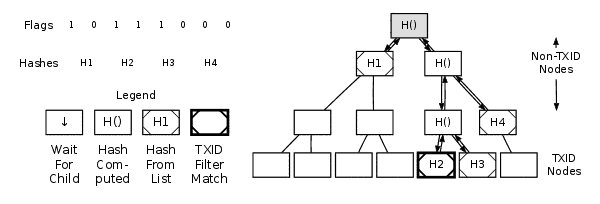
\includegraphics[width=\linewidth]{image/merkleblock-parsing}
	\caption{شکل مثال تحلیل پیام \texttt{merkleblock} در سمت کاربر سبک.\cite{P2P_ref}}
	\label{fig:merkleblock-parsing}
\end{figure}

با توجه به توضیحات بالا، گام‌های محاسبهٔ اثبات مرکل با توجه به پیام \texttt{merkleblock} دریافت شده به صورت زیر خواهد بود:

\begin{enumerate}
		\item {%
		باتوجه به اینکه تعداد تراکنش‌ها هفتا است، یک درخت مرکل سه لایه، مطابق شکل \ref{fig:merkleblock-parsing} ایجاد می‌کنیم که در ابتدا تمام گره‌های آن خالی باشد.
	}
	\item {%
		از ریشهٔ مرکل شروع می‌کنیم. مقدار اولین بیت \lr{flags} یک است. به این ترتیب مقدار گره ریشه بعدا و با توجه به مقدار بچه‌هایش مشخص می‌شود. گره بعدی مورد بررسی را بچهٔ سمت چپ ریشهٔ مرکل قرار می‌دهیم. به خاطر آن‌که گره ریشه اولین گره بررسی آن را گره شماره یک می‌نامیم.
	}

	\item {%
در این مرحله، گره مورد بررسی گره بچهٔ سمت چپ ریشهٔ مرکل است. با توجه به اینکه بیت بعدی \lr{flags} برابر صفر است، اولین چکیدهٔ استفاده نشده (\lr{Hash \#1}) را در این گره قرار می‌دهیم و دیگر کاری با گره‌های زیر دستی آن داریم. این گره را گره شمارهٔ دو می‌نامیم. به این ترتیب مطابق شکل \ref{fig:merkleblock-parsing} مقدار \lr{H1} در این گره قرار می‌گیرد. به گره بالاتر (ریشهٔ مرکل) برگشته و بچهٔ راستی آن را انتخاب می‌کنیم.
	}
	\item{%
	مقدار بیت بعدی (سوم) \lr{flags} برابر ۱ است، پس  مقدار این گره باید توسط گره‌های زیردستی آن محاسبه شود. به این ترتیب، بچهٔ سمت چپی آن انتخاب می‌شود.
}
	\item{%
	در این مرحله‌ هم مانند مرحلهٔ قبل، چون بیت چهارم \lr{flags} نیز یک است گره بچهٔ سمت چپی انتخاب می‌شود.
}
	\item{%
	در این مرحله یک گره \lr{TXID} انتخاب شده است. از آن‌جا که گره‌های مربوط به تراکنش‌ها زیرگره‌ای ندارند، مقدار آن‌ها حتما باید توسط گره کامل در اختیار گره سبک قرار گیرد. به این ترتیب مقدار چکیدهٔ استفاده نشدهٔ بعدی، یعنی \lr{Hash \#2} را در این گره قرار می‌دهیم. مقدار بیت پنجم \lr{flags} که متناظر با این گره است برابر یک بوده که این معنا را می‌رساند که این \lr{TXID} برای تراکنشی است که یکی از عناصر آن با فیلتر بلوم منطبق شده‌اند پس به گره سبک دریافت کننده مربوط است. 
}

	\item{%
	در مرحلهٔ بعدی، به گره پدر برگشته و گره بچهٔ سمت راستی انتخاب می‌شود. باز هم چون این گره، بچه‌ای ندارد و مربوط به یک \lr{TXID} است، مقدار  \lr{Hash \#3} را در آن قرار می‌دهیم. صفر بوده بیت ششم \lr{flags} به این معنا است که این تراکنش با فیلتر منطبق نشده است. ارسال آن صرفا برای اثبات مرکل نیاز است.
}

	\item{%
	به گره پدر (چهارمین گره بررسی شده) بر می‌گردیم. از آن‌جایی که اطلاعات لازم برای محاسبهٔ چکیدهٔ این گره را از دو مقدار  \lr{TXID} داده شده داریم، مقدار چکیدهٔ را محاسبه کرده و سپس گره بالاتر را انتخاب می‌کنیم. 
}
	\item{%
	در این مرحله وارد بچهٔ سومین گره می‌شویم. چون مقدار بیت هفتم \lr{flags} صفر است، چکیدهٔ \lr{Hash \#4} را درون آن قرار می‌دهیم. در این مرحله دیگر گره‌ای نیست که گره کامل مقدار آن را فرستاده باشد و بیت آخر \lr{flags} به خاطر لایی گذاری مقدار صفر دارد. 
}
	\item{%
	در مرحلهٔ آخر مقدار چکیدهٔ گره سوم و به تبع آن مقدار ریشهٔ درخت مرکل را محاسبه می‌کنیم. بررسی می‌شود که مقدار ریشهٔ محاسبه شده با مقدار ریشهٔ مرکلی که در سرایند بلوک قرار داشته است یکسان باشد.
}
\end{enumerate}

به این ترتیب گره سبک سعی می‌کند که به جای ارسال مستقیم آدرس‌هایش به یک گره کامل، آدرس‌هایش را درون یک فیلتر بلوم قرار دهد و این فیلتر با با پیام \texttt{filterload} برای یک گره کامل ارسال نماید. گره کامل عناصر متفاوتی از یک تراکنش را در فیلتر بلوم ارسال شده ارزیابی می‌کند و همچنین می‌تواند در صورت اجازهٔ گره سبک آن را به روزرسانی نماید

\paragraph{ملاحظات پیاده‌سازی}
بیت‌کوین‌جی\cite{bitcoinj} به صورت پیش‌فرض، نرخ خطای نوع دو را برابر $0.1$ درصد قرار می‌دهد. در پیاده‌سازی گره سبک بیت‌کوین‌جِی برای هر آدرس، کلید عمومی و چکیده کلید عمومی (آدرس) گذاشته می‌شود. پس به ازای یک آدرس بیت‌کوین، دو عنصر در فیلتر بلوم گذاشته می‌شود. این موضوع یک آسیب‌پذیری ایجاد خواهد کرد که به گره متخاصم این امکان را می‌دهد که در صورتی که متوجه شود یک \lr{PubKey} در فیلتر بلوم قرار دارد، مقدار چکیده (\lr{PubKeyHash}) آن  را نیز امتحان می‌کند. اگر مقدار چکیده هم در فیلتر بلوم قرار داشت، با اطمینان بیشتر می‌تواند مطمئن شود که این آدرس یکی از آدرس‌های کاربر سبک استفاده کننده از فیلتر بلوم است. قطعه کد زیر بخشی از پیاده‌سازی فیلتر بلوم در کد بیت‌کوین‌جِی است\cite{bitcoinj_BloomFilter}.


\lr{
	\texttt{/** Inserts the given key and equivalent hashed form (for the address). */\\
		public synchronized void insert(ECKey key) \{\\
		insert(key.getPubKey());\\
		insert(key.getPubKeyHash());\\
		\}\\}
}


در پایان‌نامهٔ\cite{Nick2015}، با هدف پیدا کردن آدرس‌های نهفته شده در این فیلتر بلوم با استفاده از این آسیب‌پذیری، از تاریخ $12$ دسامبر $2014$ الی $10$ فوریه $2015$، یک گره کامل راه‌اندازی شده و شروع به جمع‌آوری $70,078$ فیلتر کرده است که آن‌ها از گره‌های سبک دریافت نموده است. علاوه بر در این پایان‌نامه، مجموعه‌ای از تمام کلید عمومی‌ها (\lr{PubKey}) و چکیدهٔ کلید عمومی (\lr{PubKeyHash}) متناظر آن که در زنجیرهٔ بلوکی مورد استفاده قرار گرفته‌اند جمع‌آوری شده است. در نهایت همهٔ آن‌ها را با تمام فیلتر‌های بلوم جمع شده تطبیق می‌دهد. اگر هر جفت کلید عمومی و چکیدهٔ آن در فیلتر قرار داشت، نتیجه گرفته می‌شود که آن آدرس در آن فیلتر قرار دارد. در نهایت این پایان‌نامه توانست به $55,111$ جفت کلید عمومی و چکیدهٔ آن برسد که در یک فیلتر بلوم منطبق هستند.

هرچند که این ایراد به نظر ایراد پیش و پا افتاده‌ای می‌آید اما در صورتی که بیت‌کوین‌جی کلید عمومی‌ها را در فیلتر قرار ندهد، در نتیجه کیف پول نمی‌تواند از تراکنش‌هایی که خروجی آن‌ها \lr{P2PK} است مطلع شود. در حالی که، بیت‌کوین‌جی می‌خواهد از تمام انواع تراکنش‌ها پشتیبانی کند. به خاطر همین باتوجه به آگاه بودن به وجود این مشکل، اقدامی برای برطرف کردن آن تا حالا انجام نشده است.

علاوه بر مشکل ذکر شده، استفاده از فیلتر بلوم در شبکهٔ همتا‌به‌همتای بیت‌کوین با آسیب‌پذیری‌ها و چالش‌های بیشتری به مواجه است که عملا این ابزار را برای حفظ حرم خصوصی کاربران سبک بلااستفاده کرده است. در بخش \ref{Vulnerabilities} به بررسی این ضعف‌ها پرداخته شده است.

\subsubsection{آسیب‌‌پذیری‌ها }
\label{Vulnerabilities}
مقالهٔ \cite{Gervais2014} به طور مفصل به بررسی آسیب‌پذیری‌های موجود در فیلتر بلوم استفاده شده در شبکهٔ همتا‌به‌همتای بیت‌کوین پرداخته است. در این مقاله توضیح داده شده است که فیلتر بلوم نشت اطلاعاتی بسیار زیادی دارد که این نشت به تعداد آدرس‌هایی که یک کاربر دارد وابسته است. اگر فیلتر بلوم تعداد متوسطی (مثلا $10$ آدرس) از آدرس‌ها را در خود جایی دهد، مهاجم می‌تواند با احتمال خوبی آدرس‌های کاربر سبک مرتبط با آن را درست حدس بزند. به عنوان مثال احتمال درست حدس زدن آدرس‌های فیلتر بلوم با $10$ آدرس برابر $0.99$ است. 

علاوه بر این حتی اگر تعداد آدرس‌ها در فیلتر‌ بلوم افزایش پیدا کند، در حالی که مهاجم بتواند به دو فیلتر بلوم مربوط به یک کاربر سبک دست پیدا کند، قادر خواهد بود که با دقت بالایی آدرس‌های مربوط به کاربر سبک را تشخیص دهد. چرا که اگر یک گره کامل متخاصم دو فیلتر بلوم متفاوت از یک کیف پول را در دست داشته باشد، می‌تواند با وارد کردن عناصر به هر دو فیلتر، تا حد قابل ملاحظه‌ای خطاهای نوع دوم را برطرف نماید\cite{Nick2015}. لازم به ذکر است که در پیاده‌سازی‌های فعلی با راه‌اندازی مجدد گره سبک، فیلتر بلوم تغییر می‌کند و به گره کامل متخاصم شانس دسترسی به فیلتری‌های بلوم متعددی از یک کاربر سبک را می‌دهد\cite{Gervais2014} زیرا مقدار تصادفی \lr{nTweak} متفاوتی استفاده خواهد کرد.

در مقالهٔ \cite{Gervais2014}، به معرفی یک معیار برای سنجش حریم خصوصی  فیلتر بلوم پرداخته است. این معیار اینطور تعریف می‌شود که 
$P_{h_{(j)}}$
 برابر است با احتمال آن‌که یک متخاصم ‌$j$ عنصری که واقعا در فیلتر بلوم قرار گرفته اند را که فرد متخاصم اطلاعاتی در مورد آن‌ها نداشته است، درست حدس بزند. محاسبهٔ $P_{h_{(j)}}$ به صورت زیر است:
%N_v = S
 \begin{equation}
 \label{eq:P_h}
 P_{h_{(j)}} = \prod_{k=0}^{j-1}\frac{N-k}{N+N_v-k} = \frac{N}{N+N_v}\cdot\frac{N-1}{N+N_v-1} \ldots
 \end{equation}
  
  که در آن $N$ تعداد آدرس‌هایی است که در بیت‌کوین قرار داده شده است. از آن‌جایی که هم \lr{PubKey} و هم \lr{PubKeyHash} درون فیلتر بلوم قرار می‌گیرند تعداد عناصر قرار گرفته در فیلتر بلوم برابر $m=2N$ است. $N_v$ هم تعداد اعضای مجموعه‌ٔ عناصری است که به خاطر خطای نوع دو با فیلتر بلوم منطبف می‌شوند. با توجه به معادلهٔ \ref{eq:P_h} احتمال آن‌که کاربر متخاصم تمام آدرس‌هایی که در حقیقت درون فیلتر بلوم $B$ هستند را به درستی حدس بزند، برابر 
  $P_{h_{(N)}} = \prod_{k=0}^{N-1}\frac{N-k}{N+N_v-k} = \frac{N!N_v!}{(N+N_v)!}$
  خواهد بود\cite{Gervais2014}. بدیهی است که هر چه مقدار $P_{h_{(.)}}$ بیش‌تر باشد،‌ فیلتر بلوم حریم خصوصی را کمتر حفظ می‌کند.
  
  

آسیب‌پذیری دیگر آن‌ است که در کاربرد‌های حفظ حریم خصوصی با استفاده از فیلتر بلوم، لازم است که به این مسئله توجه شود که اگر با قرار دادن آدرس $x$ در فیلتر بلوم، تعدادی بیت یک شود به طوری که نتوان آن بیت‌ها را با قرار دادن عناصری غیر عضو در فیلتر بلوم یک نمود، امکان حاشا کردن آنکه x در آدرس‌های مطلوب کاربر سبک قرار دارد، ممکن نخواهد بود. به بیان ساده‌تر اگر گره کامل متوجه شود که فقط به ازای یک آدرس $x$ خاص، خروجی توابع چکیده‌ساز به یک یا چند بیت مشخص نگاشت می‌شوند، می‌فهمد که حتما آدرس  $x$ جزء آدرس‌های اصلی قرار گرفته در فیلتر بلوم بوده است و گره سبک نمی‌تواند وجود آن آدرس را «حاشا» کند.

مقاله \cite{Bianchi2012} ضمن اشاره به این آسیب‌پذیری، معیاری برای سنجش حریم خصوصی فیلتر بلوم با توجه به احتمال آنکه بیت‌های یک شده در فیلتر بلوم توسط عناصر غیر عضو پوشش داده شوند، ارائه کرده است که در بخش \ref{gamma-deniability} به آن پرداخته شده است.






\section{مروری بر ادبیات موضوع}
\label{LitReview}

در این قسمت به مروری بر کارهایی که تا کنون در این حوزه انجام شده است، اشاره می‌شود:

\subsection{معیار 
	حاشاپذیری-$\gamma$ برای
	سنجش حریم خصوصی فیلتر بلوم}
\label{gamma-deniability}

در مقاله \cite{Bianchi2012} معیاری کمّی، بر اساس مدل گمنامی-$K$ 
\cite{Sweeney2002}،
برای اندازه‌گیری حریم خصوصی فیلتر بلوم معرفی شده است. در این مقاله بیان شده است که احتمال خطای نوع دو ($P_f$) به تنهایی معیار مناسبی برای سنجش حریم خصوصی فیلتر بلوم نیست. بلکه باید تعداد عناصر خطای نوع دو ($N_v$) مورد بررسی قرار گیرد. واضح است که اندازهٔ $N_v$ علاوه بر $P_f$ وابسته به تعداد کل عناصر ($N_u$) است:
$N_v=(N_u-m)\times P_f$.
با توجه به این موضوع، مقاله \cite{Bianchi2012} با بهره‌برداری از نسخهٔ احتمالاتیِ مدل گمنامی-$K$
\cite{Lodha2008}،
یک معیار سنجش گم‌نامی مناسب فیلتر بلوم ارائه داده است. عنوان این معیار «حاشاپذیری-$\gamma$» است. 

هرچند که در فیلتر بلوم، داده به صورت تجزیه ناپذیر ذخیره می‌شود و در گمنامی-$K$ داده به صورت ساختاریافته و دارای ویژگی‌های مشخصی هست، می‌توان شباهت‌های نزدیکی بین آن‌ها در نظر گرفت. به طور شهودی می‌توان این گونه تعبیر کرد که بیت‌های فیلتر ($b[i]$ و $i\in[0,n-1]$) «ویژگی‌های» عنصر $x$ هستند. یعنی، عنصر $x$ دارای ویژگی $b[i]$ است، اگر و تنها اگر به ازای حداقل یک 
$j\in[1,k]$ داشته باشیم 
$H_j(x)=i$.
به این ترتیب می‌توانیم از تعریف گمنامی-$K$ در فیلتر بلوم استفاده نماییم. عنصر $x$، قرار گرفته در فیلتر، گمنام-$K$ یقینی است اگر به ازای تمام بیت‌های $b[i]$  که توسط این عنصر یک شده‌اند، حداقل $K-1$ عنصر خطای نوع دو وجود داشته باشد که به همان بیت‌ها نگاشت شوند.

می‌توان از این تعریف فهمید که برقراری شرایط گمنامی-$K$ یقینی همیشه امکان‌پذیر نیست. از این رو، استفاده از تعمیم احتمالاتی گمنامی-$K$ 
\cite{Lodha2008} 
برای فیلتر بلوم مناسب‌تر است. به این ترتیب مقالهٔ \cite{Bianchi2012} برای عنصری که به فیلتر بلوم اضافه شده است، از صفت «حاشاپذیر» استفاده کرده است.  به این معنی که آیا دارنده فیتلر می‌تواند وجود آن عنصر در فیلتر را انکار نماید یا خیر. به این ترتیب می‌گوییم عنصر $x\in \mathcal{S}$ حاشاپذیر است اگر به ازای 
$\forall i \in \{1..k\}$،
حداقل یک عنصر از مجموعه پنهان‌سازی $v\in \mathcal{V}$ (خطای نوع دو) وجود داشته باشد به گونه‌ای که 
$\exists j \in \{1..k\}$
به شرطی که 
$H_i(x) = H_j(v)$.
به بیان ساده‌تر یک عنصر حاشا‌پذیر است اگر بتوان بدون تغییر بیت‌های فیلتر، آن عنصر را توسط عناصری که عضو فیلتر نیستند جایگذاری کرد. 

فیلتر بلوم $B$، حاشاپذیر-$\gamma$ است (یا دارای ویژگی حاشاپذیری-$\gamma$) است، هر گاه یک عنصر تصادفی آن $x\in \mathcal{S}$ با احتمال $\gamma$ حاشاپذیر باشد. احتمال تقریبی حاشاپذیری-$\gamma$ فیلتر $B$ به صورت معادله \eqref{eq:gamma-deniability} محاسبه می‌شود  \cite{Bianchi2012}.

\begin{equation}
\gamma \left(B\right) \approx \left(1-exp\left(-\frac{N_vk}{n\left(1-e^{-km/n}\right)}\right)\right)^k
\label{eq:gamma-deniability}
\end{equation}

که در آن 
$N_v=(N_u-m)\times P_f$.
هرچه مقدار $\gamma$ به یک نزدیک‌تر باشد، سطح بهتری از حریم خصوصی مُهیا شده است.
شکل \ref{fig:gamma_deniability} مثالی را نشان می‌دهد که در آن   
$\mathcal{S} = \{x_1, x_2, x_3\}$ 
مجموعه عضو فیلتر بلوم است. مجموعهٔ پنهان‌سازی (خطای نوع دو)، شامل عناصر 
$\mathcal{V} = \{v_1, v_2, v_3\}$
می‌شود. عنصر $x_1$ حاشا‌پذیر است چرا که بیت‌های مرتبط با آن، یعنی $b[0]$، $b[2]$ و $b[7]$، توسط عناصر $v_1$ و $v_2$ پوشانده شده است. به همین ترتیب می‌توان نشان داد که عنصر $x_2$ نیز حاشا‌پذیر است. اما عنصر $x_3$ حاشا‌پذیر نیست. چرا که بیت $b[8]$ توسط هیچ‌کدام از عناصر مجموعهٔ پنهان‌سازی پوشانده نشده است. به این ترتیب، این فیلتر به صورت کلی، حاشاپذیر-$0.66$ است.


\begin{figure}
	\centering
	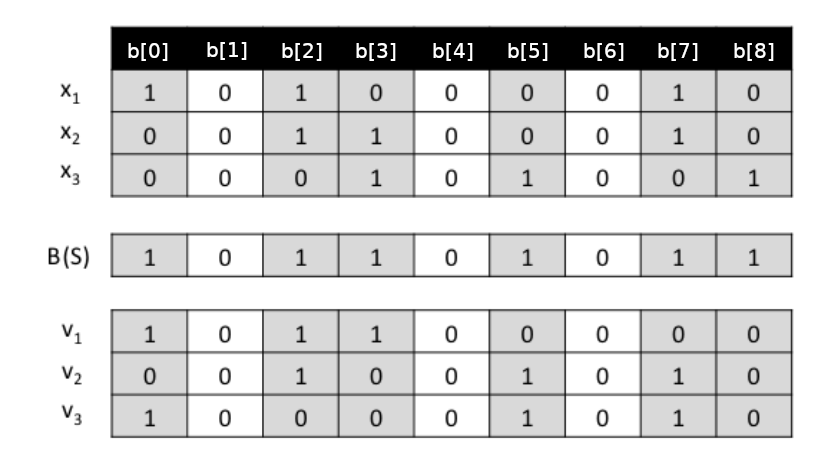
\includegraphics[width=0.8\linewidth]{image/gamma_deniability}
	\caption[مثالی از حاشاپذیری-$\gamma$]{
		یک فیلتر بلوم تشکیل شده از عناصر $\{x_1, x_2, x_3\}$ که سه عنصر $\{v_1, v_2, v_3\}$ را به عنوان خطای نوع دو می‌پذیرد\cite{Bianchi2012}.
		
	}
	\label{fig:gamma_deniability}
\end{figure}

در \cite{Kanemura2017} پیشنهاد داده است که فیلتر بلوم استفاده شده در پروتکل بیت‌کوین با توجه به معیار حاشاپذیری-$\gamma$  
\cite{Bianchi2012}،
ساخته شود. زیرا نرخ خطای نوع دو ($P_t$) به تنهایی برای سنجش حریم خصوصی فیلتر بلوم ساخته شده کافی نیست. به این ترتیب لازم است که طبق معادله \eqref{eq:gamma-deniability} در هر لحظه باتوجه به تعداد آدرس‌های یکتایی که از نقطه بررسی تا آخرین بلوک استخراج شده در زنجیره بلوکی نمایان شده‌اند ($N_u$) و $\gamma$، مقدار $P_t$ تعیین گردد. از آن‌جایی که محاسبه $N_u$ برای گره سبک غیرممکن است، در \cite{Kanemura2017} پیشنهاد شده است که از تکنیک رگرسیون خطی برای تخمین  $N_u$  استفاده شود. ضرایب مدل رگرسیون خطی، باید متناوبا (مثلا به صورت هفتگی) محاسبه گردد. این محاسبه می‌تواند به توسعه دهندگان نرم‌افزار که طرح ارائه شده در \cite{Kanemura2017}  را پیاده‌سازی می‌کنند، سپرده شود. به این ترتیب گره سبک می‌تواند مقدار $P_t$ را به نحوی تعیین کند که از امنیت فیلتر بلوم مطمئن گردد.

روش ارائه شده در \cite{Kanemura2017} دارای اشکالاتی است. یکی از اصلی‌ترین این اشکالات به روزرسانی متناوب فیلتر بلوم باتوجه به تخمین حاصل از $N_u$  است. طبق مقاله \cite{Gervais2014}، اگر گره کامل متخاصم به دو فیتلر بلوم که مربوط به یک گره سبک هستند دست پیدا کند، می‌تواند با دقت بیش‌تری آدرس‌های مربوط به گره سبک را حدس بزند. از این رو تولید متناوب فیلتر بلوم می‌تواند حریم خصوصی کاربر سبک را به خطر بیاندازد.
از ایرادات دیگر این روش می‌توان به افزایش $P_t$ در نتیجه به کار گیری از این طرح اشاره نمود. به این ترتیب، پهنای باند مورد نیاز زیادتر می‌شود. 

\subsection{فیلترکردن بلوک سمت کاربرسبک}
\label{BIP157}
در \cite{Osuntokun2017} پیشنهاد شده است که بر خلاف آن‌که گره سبک فیلتر بلوم را تولید کند و برای گره کامل ارسال نماید، گره کامل یک فیلتر از روی تمام دادگان یک بلوک ایجاد می‌کند. گره سبک به ازای هر بلوک جدید، فیلتر مربوطه را از گره کامل دریافت کرده و خودش بررسی می‌کند که آیا داده مورد نظرش در آن قرار دارد یا نه. اگر داده مورد نظر گره سبک در آن فیلتر قرار داشت، تمام بلوک را از گره کامل دریافت می‌کند.

\subsection{بازیابی اطلاعات خصوصی}
\label{PIR}
در مقاله \cite{Qin2019} از روش بازیابی اطلاعات خصوصی (PIR) جهت دریافت اطلاعات تراکنش‌ها از گره‌ کامل استفاده کرده است. بازیابی اطلاعات خصوصی به کاربران این امکان را می‌دهد که از یک پایگاه داده یا مجموعه‌ای از آن‌ها یک پرسمان انجام دهند، به گونه‌ای که سرور پایگاه داده نتواند اطلاعاتی راجع‌به کاربران درخواست دهنده و درخواست آن‌ها کسب نماید. در مقاله \cite{Qin2019}  از ترکیبی از دو رده بازیابی اطلاعات خصوصی، یعنی بازیابی اطلاعات خصوصی نظریه اطلاعاتی (IT-PIR) و محاسباتی (C-PIR) استفاده کرده است. این ترکیب در مقاله \cite{Devet2014} معرفی شده است. در ،C-PIR پرسمان توسط کاربر به نحوی کدگذاری می‌شود که پایگاه داده پاسخ مناسب را در اختیار کاربر قرار دهد اما چیزی از پرسمان و اطلاعات ذخیره شده متوجه نشود. تضمین این حریم خصوصی بر مبنای این فرض است که با اختیار داشتن توان پردازشی محدود، حل برخی مسئله‌ها  غیر ممکن یا سخت خواهد بود \cite{Devet2014}.

رده IT-PIR وابسته به فرض سخت بودن حل الگوریتم‌های پایه رمز نگاری با منابع محاسباتی محدود نیست. پروتکل‌های رده IT-PIR از چند سرور به صورت همزمان استفاده می‌کند. تا زمانی که سرورهایی که تبانی نمی‌کنند از یک تعدادی بیش‌تر باشد، حریم خصوصی کاربر تضمین می‌شود \cite{Devet2014}. 

یکی از نقص‌های IT-PIR آن است که در عمل راه حلی وجود ندارد که بتوان حداقل تعداد سرورهایی که تبانی نکنند را تامین کرد. به ویژه که یک سرور می‌تواند در شبکه حمله سیبیل\RTLfootnote{\lr{Sybil attack}}
را انجام دهد. از طرف دیگر یکی از نقص‌های اساسی C-PIR آن است که به خاطر آن‌که تنها وابسته به یک سرور است، امکان تشخیص پاسخ‌های ناقص یا غیر صحیح از طرف سرور پایگاه داده وجود ندارد \cite{Qin2019}. به بیان ساده‌تر، در کاربرد فعلی سروری که قرار است اطلاعات مربوط به زنجیره بلوکی را در اختیار کاربران سبک قرار دهد،‌ می‌تواند از انشعابی نامعتبر از زنجیره بلوکی استفاده نماید. چون گره سبک با گره‌های کامل دیگر ارتباط ندارد، نمی‌تواند متوجه این مشکل شود.

مقاله \cite{Qin2019} با استفاده از از روشی که در \cite{Devet2014} معرفی شده، از هر دوی  IT-PIR و  C-PIR استفاده کرده است. از این طریق به نقاط قوت هر دو روش دست پیدا کرده و تا حدی نقاط ضعف آن‌ها را برطرف کرده است. روش‌های بازیابی اطلاعات خصوصی عموما سرعت پایین و پیچیدگی محاسباتی بالا و همچنین مصرف پهنای باند بالایی دارند. در روش ارائه شده  \cite{Qin2019} برای رفع این مشکل، پایگاه‌های داده‌ در سه دسته هفتگی، ماهانه (احتمالا
$30$
روزه) و تمام-مدت نگهداری می‌شوند. از این طریق تاخیر و پهنای باند مصرفی برای گره‌های سبکی که نیاز به دریافت و ارزیابی تراکنش‌های جدید دارند، کاهش می‌یابد. در این روش به ازای اضافه شدن هر بلوک جدید به زنجیره بلوکی، اطلاعات بلوک جدید به دسته هفتگی اضافه می‌شود. بعد از پایان یک هفته (اضافه شدن $1008$ بلوک)، دسته هفتگی خالی شده و تمام اطلاعات آن به دسته ماهانه اضافه می‌شود. بعد از آنکه دسته ماهانه تکمیل شد (اضافه شدن $4320$ بلوک برای $30$ روز) اطلاعات آن به دسته تمام-مدت اضافه می‌شود. 


روش ارائه شده در \cite{Qin2019} مشکلاتی به همراه دارد، اول از همه آن‌که این روش نسبت به روش فیلتر بلوم \cite{Hearn2013} به صورت قابل ملاحظه‌ای پهنای باند بیشتری مصرف می‌کند. به عنوان مثال برای آنکه یک کاربر بخواهد اطلاعات یک تراکنش را که در دسته تمام-مدت قرار دارد، دریافت کند، لازم است $64.53$ مگابایت پهنای باند مصرف نماید؛ در حالی که در صورتی که از روش مرسوم فیلتر بلوم استفاده نماید، لازم است که $69.32$ کیلوبایت پهنای باند مصرف کند. البته لازم به ذکر است که هر چه تعداد تراکنش‌های درخواستی افزایش پیدا کند و از دسته‌های جدیدتر پرسمان صورت گیرد، اختلاف پهنای باند مصرفی نسبت به روش فیلتر بلوم کمتر می‌شود. مثلا، برای دریافت $100$ تراکنش از دسته هفتگی، لازم است مجموعا $33$ مگابایت اطلاعات دریافت شود و در روش مرسوم فیلتر بلوم این مقدار برابر $10.09$ مگابایت است.

دوم، آن که برای انجام بازیابی اطلاعات خصوصی، سرور پایگاه داده برای هر جدول مربوط هر دسته یک فایل مانیفست ایجاد می‌کند. این فایل مانیفست شامل ابعاد پایگاه‌داده و موقعیت هر داده است. این فایل در اختیار کاربر قرار داده می‌شود. کاربر با توجه به این مانیفست می‌تواند پرسمان‌هایی ایجاد نماید به طوری که اطلاعاتی از او نزد سرور فاش نشود. با به‌روز شدن هر دسته، حتی با اضافه شدن هر اطلاعات جدیدی از زنجیره بلوکی به دسته هفتگی، نیاز است که فایل مانیفست مربوط به آن دسته به‌روز شود. به این ترتیب نیاز است که کاربر مانیفست جدید را دریافت کند. اندازه فایل مانیفست برای پرسمان از پایگاه داده‌ای که تنها شامل بایت‌ تراکنش‌ها باشد و پرسمان از طریق TXID تراکنش صورت بگیرد، به این صورت است: هفتگی: $72.45$ مگابایت، ماهانه: $218.68$ مگابایت و تمام-مدت $3.30$ گیگابایت. البته لازم به ذکر است که نویسندگان مقاله \cite{Qin2019} می‌خواهند بعدا ساز و کاری به روش ارائه شده اضافه نمایند که کاربر سبک بدون نیاز به بارگیری فایل مانیفست، برای آنکه اطلاعات مشخصی را استخراج نماید، بتواند بدون از بین رفتن محرمانگی درخواستش، اطلاعات مورد نیازش را از مانیفست ذخیره شده در گره کامل دریافت نماید.

ایراد سوم این روش آن است که روشن است پرسمان از دسته تمام-مدت همچنان زمان‌بر است. از این رو در این مقاله پیشنهاد شده است که دسته تمام مدت به زیر دسته‌‌هایی تقسیم شود.  پرسمان کاربر سبک از زیر دسته‌های کوچک‌تر می‌تواند برای گره کامل متخاصم حاوی اطلاعاتی باشد. مثلا با تحلیل زیردسته‌هایی که از آن‌ها پرسمان انجام شده است، و همچنین کشف ارتباط بین آدرس‌ها با توجه به تراکنش‌های بیت‌کوین، به بخشی از آدرس‌های مربوط به یک کاربر سبک پی برد. علاوه بر این می‌توان به این نکته اشاره کرد که آدرس‌های یک زیر دسته قاعدتا همگی نرخ استفاده یکسانی ندارند. می‌توان فرض کرد که آدرس‌های پراستفاده‌تر احتمال پرسمان بیش‌تری از طرف کاربر سبک مالک آن داشته باشند. از این رو احتمال پرسمان آدرس‌های یک زیر دسته برابر نیست و این اطلاعاتی جانبی برای حدس آدرس درخواست شده محسوب می‌شود \cite{Niu2015}. در \cite{Qin2019} اشاره شده است که اگر این زیردسته‌ها به اندازه کافی بزرگ باشند، مثلا به اندازه دسته ماهانه، کار را برای گره متخاصم برای یافتن الگویی در پرسمان‌های کاربر سبک سخت‌تر می‌کنند. از طرف دیگر خود تقسیم‌بندی زمانی نیز باعث می‌شود که گره کامل متخاصم بتواند با توجه به دسته‌های زمانی‌ای که کاربر از آن‌ها درخواست می‌دهد به اطلاعات جانبی از کاربر سبک دست پیدا کند. 


آخرین ضعفی که می‌توان برای این روش \cite{Qin2019} نام برد، آن است که در این روش زمانی که بلوک‌های ظرفیت هر دسته تکمیل شد، مثلا برای دسته هفتگی $1008$ بلوک، آن دسته خالی شده و مقادیر آن به دسته دیگر، مثلا ماهانه، منتقل می‌شود. این معماری می‌تواند مشکلاتی به همراه داشته باشد. مثلا، کاربرانی که تراکنش‌های مربوط به آن‌ها در بلوک‌های پایانی هفته در زنجیره بلوکی ثبت می‌شود، خیلی زود تراکنششان وارد دسته ماهانه می‌شود. در نتیجه لازم است برای دستیابی به اطلاعات تراکنش مربوط به خود، هر چند که مدت زمان زیادی از آن نگذشته است، از دسته ماهانه پرسمان انجام دهد و به تبع آن پهنای باند زیادی مصرف کنند. به همین ترتیب برای تراکنش‌هایی که در بلوک‌های پایانی یک ماه ثبت می‌شوند می‌توان این مشکل را متصور شد. از طرفی دیگر اگر معماری به نحوی تغییر پیدا کند که به عنوان مثال دسته هفتگی شامل $1008$ عدد از آخرین بلوک‌هایی باشد که استخراج شده‌اند و به ازای اضافه شدن هر بلوک جدید، قدیمی‌ترین بلوک این دسته را وارد دسته ماهانه شود، باعث می‌شود که بروز رسانی دسته‌های ماهانه و به همین ترتیب دسته تمام-مدت هر $10$ دقیقه انجام شود که نه تنها سربار پردازشی بسیار زیادی برای گره کامل به وجود خواهد آورد، بلکه همه فایل‌های مانیفستی که مربوط به سه دسته هستند و نزد کاربر سبک است پس از ده دقیقه منقضی می‌شوند که با توجه به اندازه‌ٔ آن‌ها، به روزرسانی مداوم آن‌ها مرقون به صرفه نخواهد بود.

\subsection{محیط اجرای قابل اعتماد}
\label{SGX}

روش BITE
\cite{Matetic2019}
، از یک محیط اجرای قابل اعتماد (مانند 
SGX\RTLfootnote{\lr{Software Guard Extensions}}
\cite{SGX})
برای حفظ حریم خصوصی کاربران سبک بهره‌گیری می‌کند. 
محیط اجرای قابل اعتماد SGX در گره‌های کامل قرار گرفته و وظیفه پاسخ دهی به درخواستِ تایید تراکنش از طرف کاربر سبک را دارد. SGX از نرم‌افزارهایی که در خارج از آن اجرا می‌شوند (حتی سیستم‌عامل) مجزا و منزوی است و می‌تواند یکپارچگی و محرمانگی داده‌ها را در مقابل گره کامل متخاصم دارنده آن حفظ نماید. در نتیجه قادر است در حفظ حریم خصوصی کاربران سبک و صحت (یک‌پارچگی) پاسخ‌ به آن‌‌ها مفید باشد. به طوری که نه تنها باعث جلوگیری از فاش شدن اطلاعات گره سبک در برابر گره کامل دارنده آن می‌گردد بلکه می‌تواند گره سبک را مطمئن کند که اطلاعات دریافتی صحیح و کامل هستند. با این حال گره کامل می‌تواند با بررسی الگوی دسترسی SGX به یک حافظه خارجی،‌ مانند پایگاه‌ دادهٔ‌ تراکنش‌ها، آدرس کاربر درخواست دهنده را حدس بزند. همچنین SGX نسبت به حملات کانال جانبی متعددی آسیب‌پذیر است. در مقاله \cite{Matetic2019} سعی شده است با بهره‌گیری از روش بازیابی اطلاعات خصوصی و تکنیک‌های حفاظت از کانال جانبی، امنیت روش پیشنهاد شده را افزایش دهد.

مقاله \cite{Matetic2019} دو نوع راه حل ارائه داده‌ است. راه حل اول پنجره پویش (\lr{Scanning Window}) و راه حل دوم پایگاه داده ناآگاهانه (\lr{Oblivious Database}) نام دارد. در هر دو روش، تصدیق از راه دور صورت می‌گیرید و یک ارتباط امن در لایه انتقال(
TLS\RTLfootnote{\lr{Transport Layer Security}})
مابین کاربر سبک و SGX برقرار می‌شود. کاربر سبک آدرس مورد نظرش را برای SGX می‌فرستد و SGX با توجه به زنجیره بلوکی تمام اطلاعات مورد نیاز جهت درستی سنجی وجود تراکنش در زنجیره بلوکی را بدست آورده و برای کاربر سبک درخواست دهنده می‌فرستد. 

در روش پنجره پویش، برای نرمالایز کردن رابطه بین اندازه پاسخ‌ و اطلاعاتی که در واقع به آن‌ها دسترسی صورت گرفته است از یک روش پویش خاص استفاده می‌شود. همان‌طور که گفته شد گره کامل متخاصم می‌تواند با بررسی الگو دسترسی SGX به حافظه، آدرس(های) درخواست داده شده را حدس بزند، در این روش قرار است از حفظ حریم خصوصی کاربر سبک از طریق پنهان‌سازی الگو‌های دسترسی به داده‌ یا بلوک اطمینان حاصل شود. هدف اصلی این روش پنهان‌سازی کامل نسبت اندازه پاسخ (نشان‌دهنده تعداد تراکنش‌های بازگردانده شده به کاربر) و تعداد بلوک‌های پویش شده است. زیرا گره کامل متخاصم می‌تواند با مقایسه اندازه پاسخ تولید شده توسط گره کامل و همچنین تعداد بلوک‌های پویش شده توسط آن به بسامد تراکنش‌هایی که مربوط به آن آدرس هستند دست پیدا کند؛ در نتجیه آدرس مورد نظر گره سبک درخواست دهنده را حدس بزند.

در شکل \ref{fig:scanningwindow} جزئیات روش پنجره پویش را، که در آن نسبت اندازه پاسخ و تعداد بلوک‌های پویش شده ثابت می‌ماند، نشان داده می‌شود. در این روش بعضا بلوک‌های بیشتری پویش می‌شوند تا نسبت اندازه پاسخ با بلوک‌های پویش شده ثابت بماند. گره کامل متخاصم تنها می‌تواند بلوک‌هایی که به آن‌ها دسترسی صورت گرفته است را شناسایی کند و چیزی درمورد آدرسی که از طرف کاربر سبک ارسال شده است و یا تراکنش‌های بازگردانده شده نمی‌داند. در این روش برای آن‌که جلوی  حمله زمانی به الگوریتم گرفته شود، می‌توان اثبات مرکل را برای تمام تراکنش‌های موجود در بلوک‌های پویش شده محاسبه کرده و به محاسبهٔ اثبات مرکل، تنها برای تراکنش‌های مورد نظر کاربر درخواست دهنده، بسنده نکرد. به این ترتیب این روش بار پردازشی بسیار زیادی را متحمل خواهد شد. از طرف دیگر اگر که گره کامل متخاصم بتواند حملات کانال جانبی دیجیتال دانه‌بندی زیاد\RTLfootnote{\lr{High-granularity digital side-channel attacks}} را اجرا نماید به طوری که بتواند مسیر اجرای برنامه را با دانه‌بندی سطح دستورات مشاهده کند، می‌تواند تراکنش‌هایی که انتخاب شده‌اند را تشخیص دهد. در این مقاله، برای مقابله با این حملات از روشی مبتنی بر \cite{Rane2015} بهره می‌گیرد که بار پردازشی الگوریتم را افزایش می‌دهد.

\begin{figure}[h]
	\centering
	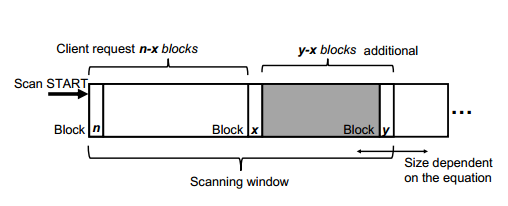
\includegraphics[width=0.7\linewidth]{image/Scanning_Window}
	\caption[پنجره پویش (\lr{Scanning Window}) ]{پنجره پویش. مطابق با تعداد بلوک‌های درخواست داده شده ($x$) و تعداد تراکنش‌های منطبق شده با درخواست مشتری در آن‌ها، احتمالا بلوک‌های بیشتری ($y$) از حافظه خوانده می‌شود تا نسبت بین بلوک‌های خوانده شده و اندازه پاسخ ثابت بماند\cite{Matetic2019}.}
	\label{fig:scanningwindow}
\end{figure}

روش دوم ارائه شده در \cite{Matetic2019} پایگاه داده ناآگاهانه نام دارد. در این روش کاربر سبک آدرس‌های مورد نظر خودش را، از طریق یک کانال محرمانه، برای SGX ارسال می‌کند و مستقیما اطلاعات مربوط به خروجی‌های خرج نشده را دریافت می‌نماید. در این روش برخلاف روش‌های پیشین و همچنین روش پنجره پویش،‌ نیاز نیست که کاربر سبک سرایند بلوک‌ها و مسیر (اثبات) درخت مرکل را دریافت و بررسی کند. در این روش کاربر به صحت عملکرد SGX و پاسخ آن اعتماد کامل دارد.
برای آنکه SGX بتواند کاربر را از صحت عملکرد خودش مطمئن سازد، 
تمام اقدامات و مقداردهی‌های اولیه به عنوان حالت اولیه ثبت می‌شود. با استفاده از آن کاربر می‌تواند مطمئن شود که کد صحیحی بر روی سامانه در حال اجرا است. به این فرایند تصدیق از راه دور\RTLfootnote{\lr{Remote Attestation}}
گفته می‌شود. تصدیق ایجاد شده، که شامل حالت اولیه است، امضا شده و برای کاربر ارسال می‌شود. کاربر می‌تواند توسط سرویس تصدیق برخطی که توسط اینتل ارائه می‌شود \cite{EPID}، امضا را بررسی نماید.

در روش پایگاه داده ناآگاهانه، SGX اطلاعات مربوط به خروجی خرج نشدهٔ تراکنش‌ها (UTXO) را در یک پایگاه داده رمزنگاری شده نگهداری می‌کند. همچنین از ماشین دسترسی تصادفی ناآگاهانهٔ
( ORAM\RTLfootnote{\lr{Oblivious Random Access Machine}})
معرفی شده در \cite{Stefanov2013} برای جلوگیری از نشت اطلاعات در هنگام دسترسی به حافظه استفاده می‌کند. به این ترتیب گره کامل متخاصم نمی‌تواند الگویی از دسترسی SGX به حافظه پیدا نماید. از طرف دیگر در این روش طول درخواست‌ها و پاسخ‌ها همواره یک مقدار ثابت است. اگر اندازه آن‌ها از آن مقدار ثابت کوتاه‌تر باشد، با لایی‌گذاری و اگر طولانی‌تر بود با تکه‌تکه کردن، به اندازه‌های ثابت تبدیل می‌شوند. در این روش SGX به تمام زنجیره بلوکی دسترسی ندارد و تنها دادهٔ UTXO را نگهداری کرده و به ازای اضافه شدن هر بلوک جدید، بعد از آن که آن بلوک را از جنبه اثبات کار و درخت مرکل درستی سنجی کرد، آن را به روزرسانی می‌کند. از آن‌جایی که UTXO در حافظه ORAM ذخیره می‌گردد، به روزرسانی آن امری نسبتا زمان‌بر، چیزی در حدود $78.5$ ثانیه، خواهد بود.

در دو روش ارائه شده در \cite{Matetic2019} بار پردازشی چندانی بر روی گره سبک قرار نخواهد گرفت. همچنین از آن‌جایی که دیگر لازم نیست برای حفظ حریم خصوصی کاربر تراکنش‌هایی مازاد به خاطر خطای نوع دو نیز دریافت شوند، پهنای باند به طور قابل ملاحظه‌ای در این دو روش نسبت به روش فیلتر بلوم کاهش پیدا می‌کند. از طرف دیگر در روش دوم (پایگاه داده ناآگاهانه) نیاز نیست که پاسخ گره کامل با اثبات‌های مرکل همراه باشد و به عبارتی گره سبک به عملکرد صحیح SGX اعتماد دارد. در نتیجه در این روش پهنای باند مصرفی بسیار کاهش پیدا می‌کند. علاوه بر مزایای ذکر شده، این روش ایراداتی نیز دارد که در ادامه به بیان آن خواهیم پرداخت.

اول از همه آنکه زمان تولید جواب در روش پنجره پویش، در صورتی که اقدامت مورد نیاز جهت جبران حمله کانال جانبی انجام شود، بسیار زمان‌بر است. به عنوان مثال برای پردازش  $100$ بلوک در این روش چیزی در حدود $73$ ثانیه زمان نیاز است. این زمان برای روش فیلتر بلوم با نرخ خطای نوع دوی $0.5$ درصد، حدود $1.1$ ثانیه است \cite{Matetic2019}. هر چند که تولید پاسخ در روش  پایگاه داده ناآگاهانه بسیار سریع‌تر انجام می‌شود، اما برای به روز رسانی داده خروجی‌ خرج نشده تراکنش‌ها نیاز به $78.5$ ثانیه زمان دارد. به عبارتی می‌توان اینطور گفت که هر ده دقیقه یک‌بار (زمان مورد نیاز برای استخراج یک بلوک جدید)، حدود یک دقیقه و هجده ثانیه،‌ صرف به روز رسانی شده و امکان پاسخ‌گویی به کاربران سبک را ندارد. مقاله \cite{Matetic2019} برای افزایش دسترس‌پذیری سیستم در شرایط به روز رسانی، پیشنهاد استفاده از دو سیستم موازی را داده است. در این شرایط نیز،‌ سیستم ارائه دهنده خدمات از وضعیت فعلی شبکه حداکثر حدود $78.5$ ثانیه عقب‌تر خواهد بود.

مشکل دیگری که روش \cite{Matetic2019} دارد، حملات فیزیکی مدرنی است که SGX نسبت به آن‌ها آسیب‌پذیر است. مثلا حملات اسپکتر\RTLfootnote{\lr{Spectre}}\cite{Kocher2019}، ملت‌داون\RTLfootnote{\lr{Meltdown}}\cite{Lipp2020} و حمله \cite{Bulck2020} که به تازگی کشف شده است، می‌توانند برای استخراج کلید‌های تصدیق از ‌SGX مورد استفاده قرار گیرند. در صورتی که گره کامل متخاصم از چنین حمله‌ای بهره‌بردای کند، می‌تواند در روش پنجره پویش، حریم خصوصی کاربران سبک درخواست دهنده را نقض نماید؛ همچنین در روش پایگاه دادهٔ ناآگاهانه علاوه بر نقض حریم خصوصی کاربر سبک می‌تواند اطلاعات اشتباهی را در اختیار وی قرار دهد.

علاوه بر مشکلات ذکر شده در بالا، می‌توان به این مسئله نیز اشاره نمود که برای آنکه یک گره کامل بخواهد خدمات پیشنهاد شده در \cite{Matetic2019} را به گره‌های سبک ارائه دهد، نه تنها نیاز است که یک محیط اجرای قابل اطمینان تهیه و راه‌اندازی نماید، بلکه لازم است که منابع پردازشی قابل توجهی را برای این منظور اختصاص دهد. در نتیجه گره‌های کاملی که بتوانند چنین خدماتی ارائه دهند، محدود خواهند بود. به تبع آن کاربران سبک مجبور خواهند بود که بین گره‌های کامل محدود‌تری انتخاب کنند که این مسئله انگیزه این گره‌های کامل را برای انجام اقدامات خصمانه بیشتر خواهد کرد. از این اقدامات می‌توان به ایجاد و دنبال کردن یک انشعاب ناصحیح از زنجیره بلوکی بیت‌کوین اشاره نمود. در حالت عادی که تعداد گره‌های کامل زیاد هستند، گره سبک می‌تواند با دریافت خدمات از گره‌های کامل متعدد از صحت اطلاعات دریافتی مطمئن گردد.

از طرف دیگر، شرکت‌های محدودی مانند اینتل، تجهیزات مربوط به یک محیط اجرای قابل اطمینان را تولید و به فروش می‌رسانند. همچنین نیاز است که برای  تصدیق از راه دور عملکرد آن‌ها به سرویس‌هایی مثل \cite{EPID} وابسته بود. به بیان دیگر می‌توان این طور گفت که برای آنکه بتوان از روش \cite{Matetic2019} بهره‌برداری کرد، لازم است به شرکت‌های محدودی اعتماد شود که این خود بر خلاف ذات شبکه‌های همتابه‌همتایی مثل بیت کوین است.



\section{نتیجه‌گیری}
‌در نتیجه‌گیری آخر این فصل، با توجه به بررسی انجام شده بر روی مراجع تحقیق، بخش‌های قابل گسترش و تحقیق در آن حیطه و چشم‌اندازهای تحقیق مورد بررسی قرار می‌گیرند.	در برخی از تحقیقات، نتیجه نهایی فصل روش تحقیق، ارائهٔ یک چارچوب کار تحقیقی 
\lr{(research framework)}
است.